\documentclass[12pt]{report}

\usepackage{setspace}

\usepackage{amsthm}

\ifdefined\HCode%
    \usepackage{amssymb}
\else
    % palatino font (doesn't work with tex4ht, but it can be specified in the CSS):
    \usepackage{newpxtext}
    \usepackage{newpxmath}
\fi

\usepackage[sort&compress,numbers]{natbib}
% \setcitestyle{maxcitenames=6}

\usepackage{array}
\usepackage{tabularx}
\usepackage{booktabs}
\usepackage{caption}
\usepackage{ragged2e}
\usepackage{microtype}
\usepackage{graphicx}
\usepackage{xcolor}
\usepackage{xparse}
\usepackage{pifont}
\usepackage{nicefrac}
\usepackage{adjustbox}
\usepackage{xspace}
% \usepackage{resizegather}

\usepackage{enumerate}
\usepackage[shortlabels]{enumitem}
\setlist[enumerate]{nosep}


\usepackage{amsmath}
% \usepackage{amssymb}
\usepackage{amsfonts}
\usepackage{slashed}
\usepackage{cancel}
\usepackage{dsfont}
\usepackage{braket}
\usepackage{multirow}
\usepackage{needspace}
\usepackage[bottom]{footmisc}
\usepackage{changepage}
\usepackage{titlesec}
\usepackage{rotating}
% \usepackage{tocloft}
\usepackage[normalem]{ulem}
\usepackage{tikz}
\usepackage[compat=1.1.0]{tikz-feynman}
\usepackage{simplewick}

\definecolor{awesome-emerald}{HTML}{00A388}
\definecolor{awesome-skyblue}{HTML}{0395DE}
\definecolor{awesome-red}{HTML}{DC3522}
\definecolor{awesome-pink}{HTML}{EF4089}
\definecolor{awesome-orange}{HTML}{FF6138}
\definecolor{awesome-nephritis}{HTML}{27AE60}
\definecolor{awesome-concrete}{HTML}{95A5A6}
\definecolor{awesome-darknight}{HTML}{131A28}
\colorlet{awesomelinks}{awesome-skyblue}

\theoremstyle{definition}
\newtheorem{definition}{Definition}[chapter]

\theoremstyle{definition}
\newtheorem{example}{Example}[chapter]

\theoremstyle{definition}
\newtheorem{theorem}{Theorem}[chapter]

\numberwithin{equation}{chapter}
% \numberwithin{figure}{section}
% \numberwithin{table}{section}

\usepackage{hyperref}
\hypersetup{colorlinks=true,
            linkcolor=awesomelinks,
            urlcolor=awesomelinks,
            citecolor=awesomelinks,}

\usepackage{doi}

\sloppy
\bibliographystyle{apsrev4-2}

% Required information
\title{Notes on Statistics for HEP}
\author{Raghav Kansal}

% Start the document
\begin{document}

\newcommand{\diag}{\ensuremath{\mathrm{diag}}\xspace}
\newcommand{\identity}{\ensuremath{\mathds{1}}\xspace}
\newcommand{\mustequal}{\ensuremath{\overset{!}{=}}\xspace}
\newcommand{\tr}[1]{\ensuremath{\mathrm{Tr}\left[#1\right]}\xspace}
\newcommand{\cnicefrac}[2]{%
  \ifdefined\HCode  % nicefrac not well supported by tex4ht
    \frac{#1}{#2}
  \else
    \nicefrac{#1}{#2}
  \fi
}
\newcommand{\cslashed}[1]{%
  \ifdefined\HCode  % slashed not supported by tex4ht
    \cancel{#1}
  \else
    \slashed{#1}
  \fi
}
\newcommand{\cvec}[1]{\mathbf{#1}}

% chi'^2
\newcommand{\chipt}{\chi^{\prime 2}}

\NewDocumentCommand{\SO}{ o }{%
  \ensuremath{\mathrm{SO}\IfValueT{#1}{(#1)}}\xspace
}
\NewDocumentCommand{\so}{ o }{%
  \ensuremath{\mathfrak{so}\IfValueT{#1}{(#1)}}\xspace
}
\NewDocumentCommand{\SU}{ o }{%
  \ensuremath{\mathrm{SU}\IfValueT{#1}{(#1)}}\xspace
}
\NewDocumentCommand{\su}{ o }{%
  \ensuremath{\mathfrak{su}\IfValueT{#1}{(#1)}}\xspace
}
\NewDocumentCommand{\UU}{ o }{%
  \ensuremath{\mathrm{U}\IfValueT{#1}{(#1)}}\xspace
}
\NewDocumentCommand{\OO}{ o }{%
  \ensuremath{\mathrm{O}\IfValueT{#1}{(#1)}}\xspace
}
\NewDocumentCommand{\EE}{ o }{%
  \ensuremath{\mathrm{E}\IfValueT{#1}{(#1)}}\xspace
}

\newcommand{\suu}{\ensuremath{\mathrm{SU}(2)\times\mathrm{U}(1)}\xspace}

\newcommand{\svecp}[1]{\ensuremath{#1_{\cvec{p}}\,}}
\newcommand{\ophat}[1]{\ensuremath{\hat #1_{\cvec{p}}\,}}
\newcommand{\ophatd}[1]{\ensuremath{\hat #1^\dagger_{\cvec{p}}\,}}

\newcommand{\abs}[1]{\left\lvert #1 \right\rvert}
\newcommand{\mus}{\ensuremath{\mu\text{s}}\xspace}
\newcommand{\mum}{\ensuremath{\mu\text{m}}\xspace}
\newcommand{\dd}{\ensuremath{\mathrm{d}}\xspace}

\newcommand{\cl}{\ensuremath{c_{\lambda}}\xspace}
\newcommand{\cvv}{\ensuremath{c_{2V}}\xspace}
\newcommand{\pt}{\ensuremath{p_{\mathrm{T}}}\xspace}
\newcommand{\Pl}{\textrm{l}\xspace}
\newcommand{\Pq}{\textrm{q}\xspace}
\newcommand{\Pg}{\textrm{g}\xspace}
\newcommand{\Pc}{\textrm{c}\xspace}
\newcommand{\Pb}{\textrm{b}\xspace}
\newcommand{\PH}{\textrm{H}\xspace}
\newcommand{\PV}{\textrm{V}\xspace}
\newcommand{\PW}{\textrm{W}\xspace}
\newcommand{\PZ}{\textrm{Z}\xspace}
\newcommand{\PQt}{\textrm{t}\xspace}
\newcommand{\PGe}{\textrm{e}\xspace}
\newcommand{\PGn}{\ensuremath{\nu}\xspace}
\newcommand{\PGm}{\ensuremath{\mu}\xspace}
\newcommand{\PGt}{\ensuremath{\tau}\xspace}
\newcommand{\PGg}{\ensuremath{\gamma}\xspace}
\newcommand{\PQq}{\textrm{q}\xspace}
\newcommand{\PQAq}{\bar{\PQq}\xspace}
\newcommand{\PQc}{\textrm{c}\xspace}
\newcommand{\PQAc}{\bar{\PQc}\xspace}
\newcommand{\PQb}{\textrm{b}\xspace}
\newcommand{\PQAb}{\bar{\PQb}\xspace}
\newcommand{\PHH}{\textrm{HH}\xspace}
\newcommand{\qqbar}{\ensuremath{\PQq\PQAq}\xspace}
\newcommand{\ccbar}{\ensuremath{\PQc\PQAc}\xspace}
\newcommand{\bbbar}{\ensuremath{\PQb\PQAb}\xspace}
\newcommand{\CL}{\textrm{CL}\xspace}
\newcommand{\CLs}{\ensuremath{\text{CL}_{\text{s}}}\xspace}

\newcommand{\PX}{\textrm{X}\xspace}
\newcommand{\PY}{\textrm{Y}\xspace}
\newcommand{\PG}{\textrm{G}\xspace}
\newcommand{\PA}{\textrm{A}\xspace}
\newcommand{\Pa}{\textrm{a}\xspace}
\newcommand{\Ph}{\textrm{h}\xspace}
\newcommand{\PHsm}{\ensuremath{\PH_{125}\xspace}}

\newcommand{\kapt}{\ensuremath{\kappa_{\PQt}}\xspace}
\newcommand{\kapl}{\ensuremath{\kappa_{\lambda}}\xspace}
\newcommand{\kapv}{\ensuremath{\kappa_{\PV}}\xspace}
\newcommand{\kapvv}{\ensuremath{\kappa_{2\PV}}\xspace}
\newcommand{\mH}{\ensuremath{m_{\PH}}\xspace}
\newcommand{\mHH}{\ensuremath{m_{\PH\PH}}\xspace}
\newcommand{\sigmaHH}{\ensuremath{\sigma_{\PH\PH}\xspace }}
\newcommand{\BR}{\ensuremath{\mathcal{B}(\HH\to\bbbar\ww)}}
\newcommand{\HH}{\ensuremath{{\PH\PH}}\xspace}
\newcommand{\HHH}{\ensuremath{{\PH\PH\PH}}\xspace}
\newcommand{\HVV}{\ensuremath{{\PH\PV\PV}}\xspace}
\newcommand{\HHVV}{\ensuremath{{\PH\PH\PV\PV}}\xspace}
\newcommand{\HHY}{\ensuremath{{\PH\PH/\PY}}\xspace}
\newcommand{\VH}{\ensuremath{{\PV\PH}}\xspace}
\newcommand{\ggH}{\ensuremath{{\Pg\Pg\PH}}\xspace}
\newcommand{\ttH}{\ensuremath{{\ttbar\PH}}\xspace}
\newcommand{\ggHH}{\ensuremath{{\Pg\Pg\PH\PH}}\xspace}
\newcommand{\qqHH}{\ensuremath{{\Pq\Pq\PH\PH}}\xspace}
\newcommand{\bbbb}{\ensuremath{\bbbar\bbbar}\xspace}
\newcommand{\mSD}{\ensuremath{m_{\text{SD}}}\xspace}
\newcommand{\ssbar}{\PQs{}\PAQs\xspace}
\newcommand{\alpS}{\ensuremath{\alpha_s}\xspace}

\newcommand{\TODO}[1]{\textcolor{red}{TODO: #1}}
\newcommand{\gbb}{\ensuremath{\Pg\to\bbbar}\xspace}
\newcommand{\hbb}{\ensuremath{\PH\to\bbbar}\xspace}
\newcommand{\hqq}{\ensuremath{\PH\to\qqbar}\xspace}
\newcommand{\htata}{\ensuremath{\PH\to\PGtp\PGtm}\xspace}
\newcommand{\qqqq}{\ensuremath{4\Pq}\xspace}
\newcommand{\ww}{\ensuremath{\PW\PW}\xspace}
\newcommand{\zz}{\ensuremath{\PZ\PZ}\xspace}
\newcommand{\VV}{\ensuremath{\PV\PV}\xspace}
\newcommand{\bbtautau}{\ensuremath{\bbbar\PGt\PGt}\xspace}
\newcommand{\bbgg}{\ensuremath{\bbbar\PGg\PGg}\xspace}
\newcommand{\bbww}{\ensuremath{\bbbar\PW\PW}\xspace}
\newcommand{\bbvv}{\ensuremath{\bbbar\PV\PV}\xspace}
\newcommand{\bbvvq}{\ensuremath{{\bbbar(\VV\to\qqqq)}}\xspace}
\newcommand{\wwq}{\ensuremath{\PW\PW\to\qqqq}\xspace}
\newcommand{\vqq}{\ensuremath{\PV\to\PQq\PQq}\xspace}
\newcommand{\VVq}{\ensuremath{\PV\PV\to\qqqq}\xspace}
\newcommand{\hvv}{\ensuremath{\PH\to\VV}\xspace}
\newcommand{\yvv}{\ensuremath{\PY\to\VV}\xspace}
\newcommand{\yww}{\ensuremath{\PY\to\ww}\xspace}
\newcommand{\hyvv}{\ensuremath{\PH/\PY\to\VV}\xspace}
\newcommand{\hyvvq}{\ensuremath{\PH/\PY\to\VV\to\qqqq}\xspace}
\newcommand{\hvvq}{\ensuremath{\PH\to\VV\to\qqqq}\xspace}
\newcommand{\yvvq}{\ensuremath{\PY\to\VV\to\qqqq}\xspace}
\newcommand{\HHbbVV}{\ensuremath{{\PH\PH\to\bbbar\VV}}\xspace}
\newcommand{\HHbbVVq}{\ensuremath{{\PH\PH\to\bbbar(\VV\to\qqqq)}}\xspace}
\newcommand{\XHY}{\ensuremath{{\PX\to\PH\PY}}\xspace}
\newcommand{\XHYbbVV}{\ensuremath{{\PX\to(\PH\to\bbbar)(\PY\to\VV)}}\xspace}
\newcommand{\XHYbbVVq}{\ensuremath{{\PX\to(\PH\to\bbbar)(\PY\to\VV\to\qqqq)}}\xspace}

\newcommand{\TXbb}{\ensuremath{T_{\mathrm{Xbb}}}\xspace}
\newcommand{\TXbbbb}{\ensuremath{T_{\mathrm{Xbb}}^{\mathrm{bb}}}\xspace}
\newcommand{\THWW}{\ensuremath{T_{\mathrm{HVV}}}\xspace}
\newcommand{\THWWww}{\ensuremath{T_{\mathrm{HVV}}^{\mathrm{VV}}}\xspace}
\newcommand{\PXbb}{\ensuremath{P_{\mathrm{Xbb}}}\xspace}
\newcommand{\PXcc}{\ensuremath{P_{\mathrm{Xcc}}}\xspace}
\newcommand{\PXqq}{\ensuremath{P_{\mathrm{Xqq}}}\xspace}
\newcommand{\PQCD}{\ensuremath{P_{\mathrm{QCD}}}\xspace}
\newcommand{\PQCDcc}{\ensuremath{P_{\mathrm{QCDcc}}}\xspace}
\newcommand{\PQCDbb}{\ensuremath{P_{\mathrm{QCDbb}}}\xspace}
\newcommand{\PQCDc}{\ensuremath{P_{\mathrm{QCDc}}}\xspace}
\newcommand{\PQCDb}{\ensuremath{P_{\mathrm{QCDb}}}\xspace}
\newcommand{\PQCDothers}{\ensuremath{P_{\mathrm{QCDothers}}}\xspace}
\newcommand{\PTop}{\ensuremath{P_{\mathrm{Top}}}\xspace}
\newcommand{\PVJets}{\ensuremath{P_{\mathrm{V+Jets}}}\xspace}
\newcommand{\PggF}{\ensuremath{P_{\mathrm{ggF}}}\xspace}
\newcommand{\PVBF}{\ensuremath{P_{\mathrm{VBF}}}\xspace}
\newcommand{\PHWWqqqq}{\ensuremath{P_{\mathrm{HVV4q}}}\xspace}
\newcommand{\PHWWqqq}{\ensuremath{P_{\mathrm{HVV3q}}}\xspace}

\newcommand{\ggfbdt}{\ensuremath{\mathrm{BDT}_{\mathrm{ggF}}}\xspace}
\newcommand{\vbfbdt}{\ensuremath{\mathrm{BDT}_{\mathrm{VBF}}}\xspace}

\newcommand{\tbw}{\ensuremath{\PQt\to\PQb\PW}\xspace}
\newcommand{\tae}{\ensuremath{\PGt_{\Pe}}\xspace}
\newcommand{\tam}{\ensuremath{\PGt_{\PGm}}\xspace}
\newcommand{\tah}{\ensuremath{\PGt_{\mathrm{h}}}\xspace}

\newcommand{\mx}{\ensuremath{{m_X}}\xspace}
\newcommand{\mh}{\ensuremath{{m_H}}\xspace}
\newcommand{\my}{\ensuremath{{m_Y}}\xspace}
\newcommand{\mxmy}{\ensuremath{{\mx,\my}}\xspace}

\newcommand{\msd}{\ensuremath{{m_{\mathrm{SD}}}}\xspace}
\newcommand{\mreg}{\ensuremath{{m_{\mathrm{reg}}}}\xspace}
\newcommand{\mregbb}{\ensuremath{{m_{\mathrm{reg}}^{\mathrm{bb}}}}\xspace}
\newcommand{\mregvv}{\ensuremath{{m_{\mathrm{reg}}^{\mathrm{VV}}}}\xspace}
\newcommand{\mjj}{\ensuremath{{m^{\mathrm{jj}}}}\xspace}
\newcommand{\mjjvbf}{\ensuremath{{m^{\mathrm{jj}}_{\mathrm{VBF}}}}\xspace}
\newcommand{\detajjvbf}{\ensuremath{{|\Delta\eta^{\mathrm{jj}}_{VBF}|}}\xspace}

\newcommand{\pois}{\ensuremath{\mathrm{Pois}}\xspace}


\newcommand{\NA}{\ensuremath{\text{---}}\xspace}
\newcommand{\kt}{\ensuremath{k_{\mathrm{T}}}\xspace}
\newcommand{\eV}{\ensuremath{\,\text{e\hspace{-.08em}V}}\xspace}
\newcommand{\MeV}{\ensuremath{\,\text{Me\hspace{-.08em}V}}\xspace}
\newcommand{\GeV}{\ensuremath{\,\text{Ge\hspace{-.08em}V}}\xspace}
\newcommand{\TeV}{\ensuremath{\,\text{Te\hspace{-.08em}V}}\xspace}
\newcommand{\unit}[1]{\ensuremath{\text{\,#1}}\xspace}
\newcommand{\GEANTfour} {{\textsc{Geant4}}\xspace}
\newcommand{\PYTHIA} {{\textsc{pythia}}\xspace}
\newcommand{\HERWIG} {{\textsc{herwig}}\xspace}
\newcommand{\SHERPA} {{\textsc{sherpa}}\xspace}
\newcommand{\ttbar}{\ensuremath{\mathrm{t}\overline{\mathrm{t}}}\xspace}
\newcommand{\MADGRAPH} {{\textsc{MadGraph}}\xspace}
\newcommand{\MCATNLO} {{\textsc{MC@NLO}}\xspace}
\newcommand{\MGvATNLO}{\MADGRAPH{}5\_a\MCATNLO\xspace}
\providecommand{\mSD}{\ensuremath{m_{\mathrm{SD}}}\xspace}
\newcommand{\rpf}{\ensuremath{R_{\mathrm{P/F}}}\xspace}


\newcommand{\etarel}{\ensuremath{\eta^{\mathrm{rel}}}\xspace}
\newcommand{\phirel}{\ensuremath{\phi^{\mathrm{rel}}}\xspace}
\newcommand{\ptrel}{\ensuremath{p_{\mathrm{T}}^{\mathrm{rel}}}\xspace}

\newcommand{\real}[1]{\ensuremath{#1_{\mathrm{real}}}\xspace}
\newcommand{\gen}[1]{\ensuremath{#1_{\mathrm{gen}}}\xspace}
\newcommand{\fgdinf}{\ensuremath{\mathrm{FGD}_\infty}\xspace}

\newcommand{\wass}{\ensuremath{W_1}\xspace}
\newcommand{\wassm}{\ensuremath{W_1^{\mathrm M}}\xspace}
\newcommand{\wassp}{\ensuremath{W_1^{\mathrm P}}\xspace}
\newcommand{\wassefp}{\ensuremath{W_1^{\mathrm{EFP}}}\xspace}
\newcommand{\wassppt}{\ensuremath{W^{\ptrel}_{1p}}\xspace}

\newcommand{\jetnet}{\textsc{JetNet}\xspace}


\newcommand{\hhexp}{69\xspace}
\newcommand{\hhobs}{142\xspace}
\newcommand{\cvvexp}{0.9\xspace}
\newcommand{\cvvobs}{1.1\xspace}
\newcommand{\kvvexplims}{\ensuremath{[0.05, 1.98]}\xspace}
\newcommand{\kvvobslims}{\ensuremath{[-0.04, 2.05]}\xspace}

\newcommand{\ri}{\ensuremath{\rho_{\mathrm{in}}}\xspace}
\newcommand{\ro}{\ensuremath{\rho_{\mathrm{out}}}\xspace}
\newcommand{\CX}{\ensuremath{\mathcal{X}}\xspace}
\newcommand{\CY}{\ensuremath{\mathcal{Y}}\xspace}


\newcommand{\parenthesis}[1]{\left( #1 \right)}
\newcommand{\squarebracket}[1]{\left[ #1 \right]}
\newcommand{\xmark}{\text{\ding{55}}}
\newcommand{\order}[1]{\mathcal{O} \left( #1 \right)}


\makeatletter
\def\lasthline{\noalign{\hrule}\noalign{\vskip-2em\vskip-\arraycolsep}}
\def\fbottomrule{\noalign{\bottomrule}\noalign{\vskip-2em\vskip-\arraycolsep}}
\makeatother

\newcommand{\cbottomrule}{%
  \ifdefined\HCode  % slashed not supported by tex4ht
    \lasthline
  \else
    \bottomrule
  \fi
}

\maketitle

\begin{abstract}
\begin{doublespace}
% \hypersetup{urlcolor=awesome-nephritis}
\setlength{\parskip}{\baselineskip}
This is a series of walk-throughs of some concepts in statistics relevant for high energy physics (HEP). 
It is primarily based on (me trying to understand) Refs.~\cite{Cowan:2010js} and~\cite{Cranmer:2014lly}, and the CMS combine tool~\cite{CMS:2024onh}.
Both references are useful and highly recommended for reading; the emphasis here is heavily on \textbf{implementing and visualizing what they discuss in Python} --- as well as providing some heuristic derivations of some of their formulae --- as that is what personally helped me build an intuition for these concepts.

These notes are primarily intended to be followed interactively \href{https://rkansal47.github.io/stats-for-hep}{online} as Jupyter notebooks, but are also available as a \href{https://github.com/rkansal47/stats-for-hep/blob/gh-pages/stats-for-hep.pdf?raw=true}{PDF}.
Feedback and corrections are very welcome through e-mail or as \href{https://github.com/rkansal47/stats-for-hep/issues}{issues} on \href{https://github.com/rkansal47/stats-for-hep/}{Github}.
Finally, for those interested, some more notes and tutorials I have written up, such as on the standard model and machine learning in HEP, are available \href{https://www.raghavkansal.com/teaching/}{here}.
\end{doublespace}
\end{abstract}


{
\hypersetup{linkcolor=black}
\tableofcontents
}

\setlength{\parskip}{\baselineskip}

\begin{doublespace}
\chapter{Introduction}

Once data is collected by high energy physics (HEP) experiments and reconstructed offline, it is analyzed to search and measure processes of interest.
Typically, the raw data is entirely dominated by irrelevant background processes which we want to filter out in favor of the signal.
The first step towards this is through appropriate online triggers, followed by offline selections to isolate the signal.

Optimizing the event selection for all but a handful of data-driven searches requires simulations of the signal and background processes.
Additionally, once the selections and phase space in which to perform the measurement have been finalized, the expected signal and background yields have to be carefully estimated, which often again necessitates simulations, as well as data-driven methods via unbiased control regions.

Once we have our observations, and signal and background estimates, the final critical step is to interpret the results in a robust statistical framework.
At the LHC, this is typically done using a frequentist, likelihood-based approach.
In these notes, this approach is introduced by way of simple experimental examples.

These notes are organized as follows.
Chapter~\ref{sec:likelihood} introduces the concepts of the likelihood functions and test statistics, with Chapter~\ref{sec:hypothesis_testing} discussing the framework for hypothesis testing, including $p$-values, significances, and the statistical definition of a ``discovery''.
Chapters~\ref{sec:intervals} and~\ref{sec:expected} then describe frequentist confidence intervals and upper limits, and the important concepts of expected significances and limits, respectively.
Finally, asymptotic approximations to simplify these computations are discussed in Part~\ref{sec:asymptotic}.


\part{Frequentist statistics at the LHC}

\chapter{The likelihood function and test statistics}
\label{sec:likelihood}

\section{The data model}
\label{sec:data_model}

Let us take the simplest possible case of a (one bin) counting experiment, where in our ``signal region'' we expect $s$ signal events and $b$ background events.
The probability to observe $n$ events in our signal region is distributed as a Poisson with mean $s+b$:
\begin{equation}
\label{eq:poisson}
P(n; s, b) = \pois(n; s+b) = \frac{(s+b)^n e^{-(s+b)}}{n!}
\end{equation}

Since we have only one observation but two free parameters, this experiment is underconstrained.
So, let's also add a ``control region'' where we expect no signal and $b$ background events.
The probability of observing $m$ events in our control region is therefore:
\begin{equation}
\label{eq:pois2}
\pois(m; b) = \frac{b^m e^{-b}}{m!}
\end{equation}
Combining the two, the joint probability distribution for $n$ and $m$ is:
\begin{equation}
\label{eq:pois3}
P(n, m; s, b) = \pois(n; s+b) \cdot \pois(m; b) = \frac{(s+b)^n e^{-(s+b)}}{n!} \cdot \frac{b^m e^{-b}}{m!}
\end{equation}
This is also called the model for the data and is plotted for sample $s, b$ values in Figure~\ref{fig:pois}.

\begin{figure}[htb]
    \centering
    \captionsetup{justification=centering}
    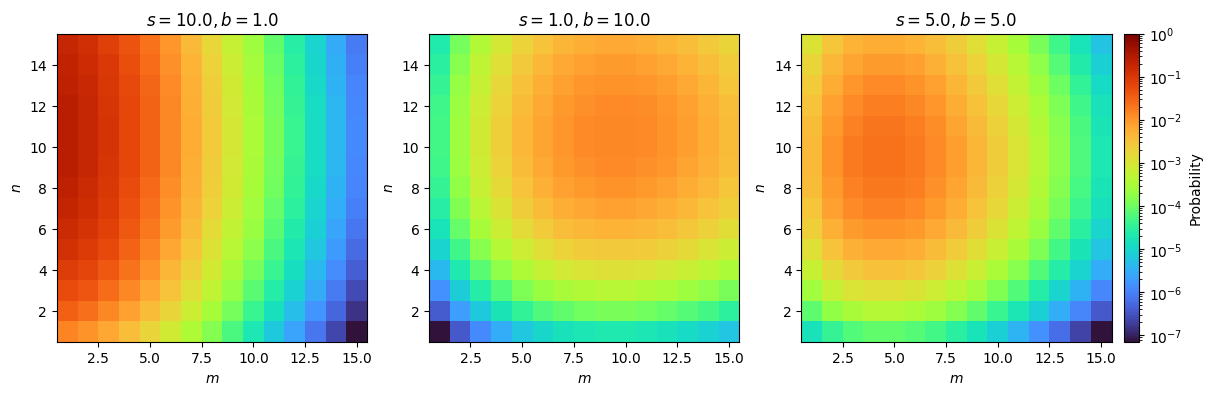
\includegraphics[width=\textwidth]{figures/01-intro/1.png}
    \caption{Sample 2D Poisson distributions.}
    \label{fig:pois}
\end{figure}

\section{The likelihood function}

In the \textit{frequentist} philosophy, however, all our parameters $n$, $m$ etc. are simply fixed values of nature and, hence, don't have a probability distribution.
Instead, we work with the \textit{likelihood function}, which is a function only of our parameters of interest (POIs), $s$ in our example, and ``nuisance parameters'' ($b$), given fixed values for $n$ and $m$:
\begin{equation}
\label{eq:likelihood}
L(s, b) = P(n, m; s, b) = \frac{(s+b)^n e^{-(s+b)}}{n!} \cdot \frac{b^m e^{-b}}{m!}.
\end{equation}
Importantly, this is not a probability distribution on $s$ and $b$! To derive that, we would have to use Bayes' rule to go from $P(n, m; s, b) \to P(s, b; n, m)$; however, such probability distributions don't make sense in our frequentist world view, so we're stuck with this likelihood formulation.
Often, it's more convenient to consider the negative log-likelihood:
\begin{equation}
\label{eq:nll}
-\ln L = \ln n! + \ln m! + s + 2b - n\ln(s+b) - m \ln b
\end{equation}

\section{The profile likelihood ratio}

Fundamentally, the goal of any experiment is to test the compatibility of the observed data ($n, m$ here) with a certain hypothesis $H$.
We do this by mapping the data to a ``test statistic'' $t$, which is just a number, and comparing it against its distribution under $H$, $P(t| H)$.
Our problem, thus, boils down to 1) choosing the most effective $t$ for testing $H$, and 2) obtaining $P(t| H)$.

In the case of testing a particular signal strength, we use the ``profile likelihood ratio'':
\begin{equation}
\label{eq:plr}
\lambda(s) = \frac{L(s, \hat{\hat{b}}(s))}{L(\hat{s}, \hat{b})},
\end{equation}
where $\hat{s}, \hat{b}$ are the maximum-likelihood estimates (MLEs) for $s$ and $b$, given the observations $n, m$, and $\hat{\hat{b}}(s)$ is the MLE for $b$ given $n, m$, \textit{and} $s$.
The MLE for a parameter is simply the value of it for which the likelihood is maximized, and will be discussed in the next section.
The numerator of $\lambda(s)$ can be thought of as a way to ``marginalize'' over the nuisance parameters by simply values that maximize the likelihood for any given $s$, while the denominator is effectively a normalization factor, such that $\lambda(s) \leq 1$.

Again, it's often more convenient to use the (negative) logarithm:
\begin{equation}
\label{eq:ts}
t_s = -2 \ln \lambda(s)
\end{equation}
% This statistic also has nice asymptotic forms, which we'll see later.
Note that $\mathrm{Max}[\lambda(s)] = 1 \Rightarrow \mathrm{Min}[t_s] = 0$.
$\lambda(s)$ and $t_s$ are plotted for sample $n, m$ values with $n - m = 10$ in Figure~\ref{fig:plr}.
The maximum (minimum) of the profile likelihood ratio ($t_s$) is at $s = n - m = 10$, as we expect; however, as the ratio between $n$ and $m$ decreases --- i.e., the experiment becomes more noisy --- the distributions broaden, representing the reduction in sensitivity, or the higher uncertainty on the true value of $s$.

\begin{figure}[htb]
    \centering
    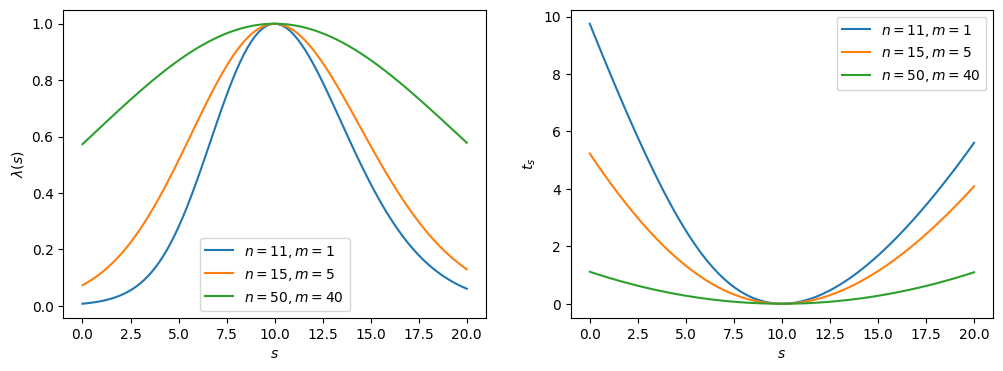
\includegraphics[width=\textwidth]{figures/01-intro/2.png}
    \caption{The profile likelihood ratio $\lambda(s)$ (left) and the $t_s$ test statistic (right) for our one-bin Poisson model.}
    \label{fig:plr}
\end{figure}

Note that the likelihood ratio and $t_s$ are also broadened due to the nuisance parameter; i.e., because we are missing information about $b$.
This can be demonstrated by plotting them with $b = m$, emulating perfect information of $b$ (Figure~\ref{fig:plr_nob}), and indeed, we see the functions are narrower than in Figure~\ref{fig:plr}.
More generally, increasing (decreasing) the uncertainties on the nuisance parameters will broaden (narrow) the test statistic distribution.
This is which is why experimentally we want to constrain them through auxiliary measurements as much as possible.

\begin{figure}[tb]
    \centering
    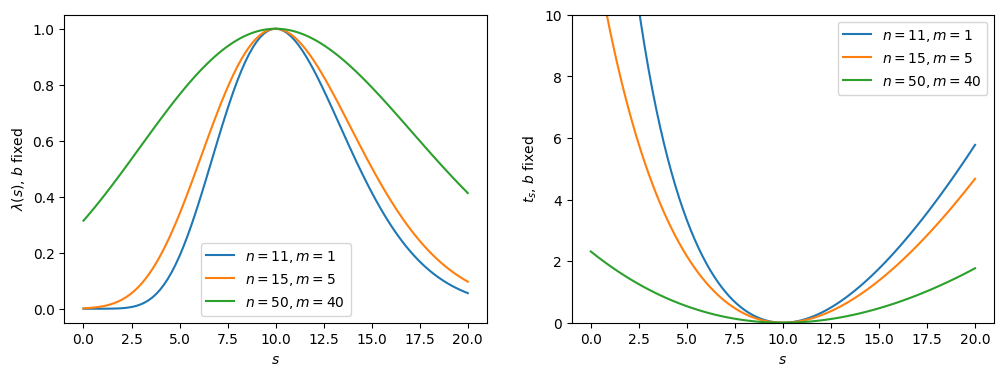
\includegraphics[width=\textwidth]{figures/01-intro/3.png}
    \caption{The profile likelihood ratio $\lambda(s)$ (left) and the $t_s$ test statistic (right) with $b = m$, demonstrating the effect of decreasing uncertainties on our nuisance parameters.}
    \label{fig:plr_nob}
\end{figure}

\section{Maximum-likelihood estimates}

MLEs for $s$ and $b$ can be found for this example by setting the derivative of the negative log-likelihood to 0 (more generally, this would require numerical minimization):
\begin{align}
\label{eq:cmle_b}
\frac{\partial (-\ln L)}{\partial s} &= 1 - \frac{n}{s+b} = 0 \\
\frac{\partial (-\ln L)}{\partial b} &= 2 - \frac{n}{s+b} - \frac{m}{b} = 0
\end{align}
Solving simultaneously yields, as you might expect:
\begin{equation}
\label{eq:mles}
\hat{b} = m, \hat{s} = n - m,
\end{equation}
Or just for $\hat{\hat{b}}(s)$ from Eq.~\ref{eq:cmle_b}:
\begin{equation}
\label{eq:cmle_b_f}
2b^2 + (2s - n - m)b - ms = 0
\end{equation}
Plugging this back in, we can get $\lambda(s)$ and $t_s$ for any given $s$.
%  (which I won't write out because even in this simple example they're painful).

% The next step would be to derive $P(t| H)$, by either sampling $t$s for multiple ``toy'' generated events or using an asymptotic (i.e., large $n,m$) approximation.

\section{Alternative test statistic}

So far, our construction allows for $s < 0$; however, physically the number of signal events can't be negative.
Rather than incorporating this constraint in the model, it's more convenient to impose this in the test statistic, by defining:
\begin{equation}
    \tilde{\lambda}(s) = \left\{
    \begin{array}{ll}
      \frac{L(s, \hat{\hat{b}}(s))}{L(\hat{s}, \hat{b})}, & \mbox{$\hat{s}\geq0$}.\\
      \frac{L(s, \hat{\hat{b}}(s))}{L(\hat{0}, \hat{\hat{b}}(0))}, & \mbox{$\hat{s}<0$}.
    \end{array}
  \right.,
\label{eq:lambda_tilde}
\end{equation}
and
\begin{equation}
    \tilde{t}_s = -2\ln \tilde{\lambda}(s)
\label{eq:t_tilde}
\end{equation}

The difference between the nominal and alternative test statistics is highlighted in Figure~\ref{fig:alt_ts}.
For $n < m$, the $\tilde{\lambda}(s) = 1$ and $\tilde{t}_s = 0$ values are at $s = 0$, since physically that is what fits best with our data (even though the math says otherwise).

\begin{figure}[htb]
\centering
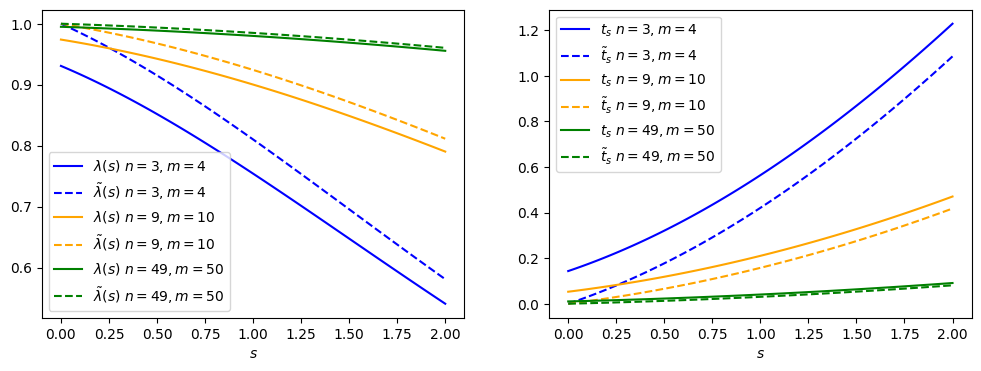
\includegraphics[width=\textwidth]{figures/01-intro/4.png}
\captionsetup{justification=centering}
\caption{Comparing the nominal vs alternative test statistic.}
\label{fig:alt_ts}
\end{figure}

Next, we want to translate this to a probability distribution of $\tilde{t}_s$ under a particular signal hypothesis ($H_s$) (i.e., an assumed value of $s$): $p(\tilde{t}_s|H_s)$, or just $p(\tilde{t}_s|s)$ for simplicity.


\chapter{Hypothesis testing}
\label{sec:hypothesis_testing}

The goal of any experiment is to test whether our data support or exclude a particular hypothesis $H$, and quantify the (dis)agreement. For example, to what degree did our search for the Higgs boson agree or disagree with the standard model hypothesis?

We have already discussed the process of mapping data to a scalar test statistic $t$ that we can use to test $H$.
However, we need to know the probability distribution of $t$ under $H$ to quantify the (in)consistency of the observed data with $H$ and decide whether or not to exclude $H$.

We must also recognize that there's always a chance that we will exclude $H$ even if it's true (called a Type I error, or a false positive), or not exclude $H$ when it's false (Type II error, or false negative).
The probability of each is referred to as $\alpha$ and $\beta$, respectively.
This is summarized handily in Table~\ref{tab:error_types}.

\begin{table}[htb]
\centering
\captionsetup{justification=centering}
\caption{Table of error types, reproduced from Ref.~\cite{enwiki:1259353735}.}
\label{tab:error_types}
\renewcommand{\arraystretch}{1.5} % Increase vertical spacing
\begin{tabular}{c|c|c|c}
\toprule
\multicolumn{2}{c|}{\multirow{2}{*}{Table of error types}} & \multicolumn{2}{c}{Null hypothesis ($H_0$) is} \\ \cline{3-4}
\multicolumn{2}{c|}{} & True & False \\
\midrule
\multirow{2}{*}{\raisebox{-1.25cm}{\begin{tabular}[c]{@{}c@{}}Decision\\ about null\\ hypothesis ($H_0$)\end{tabular}}} & Fail to reject & \begin{tabular}[c]{@{}c@{}}Correct inference\\ (true negative)\\ (probability = $1-\alpha$)\end{tabular} & \begin{tabular}[c]{@{}c@{}}Type II error\\ (false negative)\\ (probability = $\beta$)\end{tabular} \\ \cline{2-4}
    & Reject & \begin{tabular}[c]{@{}c@{}}Type I error\\ (false positive)\\ (probability = $\alpha$)\end{tabular} & \begin{tabular}[c]{@{}c@{}}Correct inference\\ (true positive)\\ (probability = $1-\beta$)\end{tabular} \\
\cbottomrule
\end{tabular}
\end{table}


Before the test, we should decide on a probability of making a Type I error, $\alpha$, that we are comfortable with, called a ``significance level''. Typical values are 5\% and 1\%, although if we're claiming something crazy like a new particle, we better be very sure this isn't a false positive; hence, we set a much lower significance level for these tests of $3\times10^{-7}$.
(The \textit{significance} of this value will be explained in Section~\ref{sec:significance} below.)

\section{Deriving \texorpdfstring{$p(\tilde{t}_s|s)$}{p(ts|s)}}

We can approximate $p(\tilde{t}_s|s)$ by generating several pseudo- or ``toy'' datasets assuming $s$ expected signal events.
In this case, this means sampling possible values for $n, m$ from our probability model.
We will continue with our simple counting experiment (Section~\ref{sec:data_model}), for which such toy datasets are generated and then used to create histograms for $p(\tilde{t}_s|s)$ in Figure~\ref{fig:p_tilde_t}.
Note that one complication in generating these toys is that the $n, m$ distributions from which we want to sample (Eq.~\ref{eq:pois3}) also depend on the nuisance parameter $b$.
However, we see from the figure that this does not matter as much as we might expect.

\begin{figure}[htb]
\centering
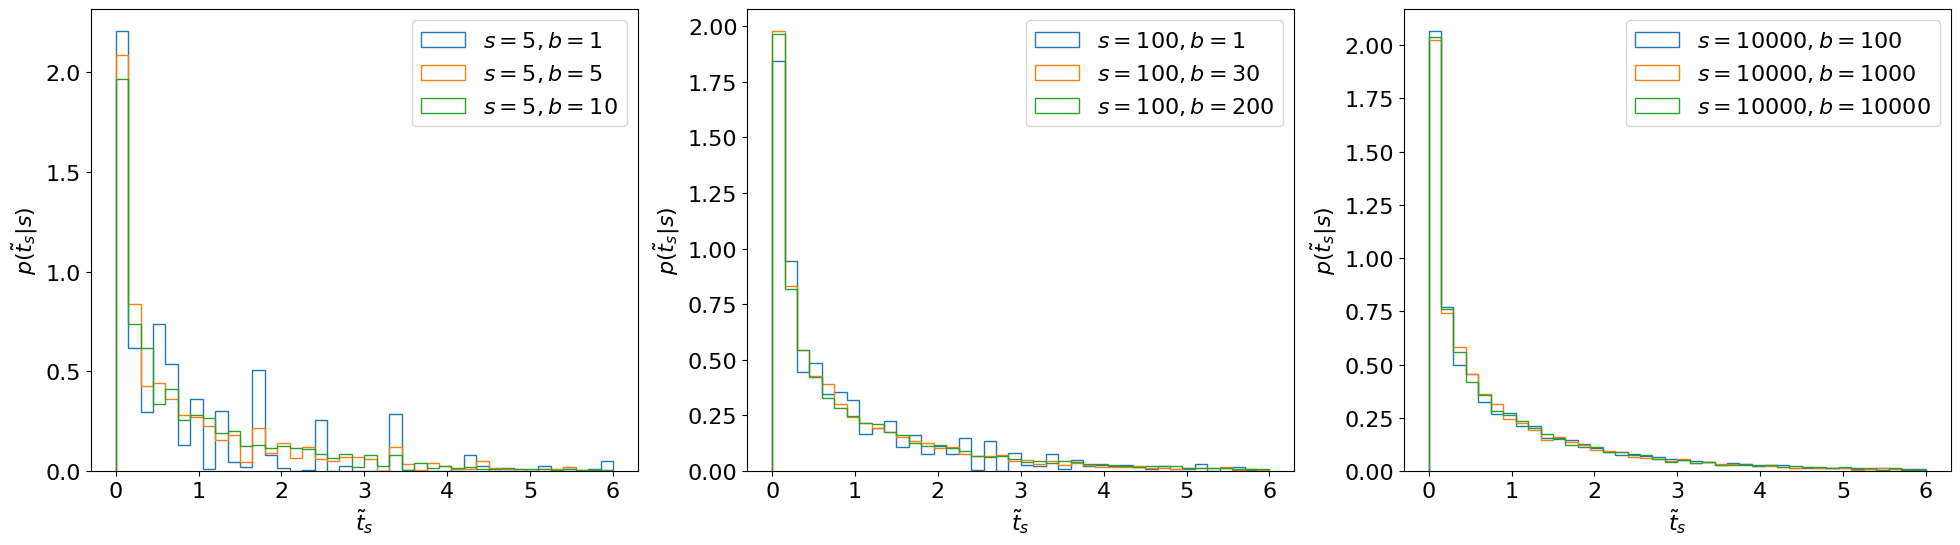
\includegraphics[width=\textwidth]{figures/02-hypothesis-testing/1.png}
\captionsetup{justification=centering}
\caption{Estimating $p(\tilde{t}_s|s)$ through toys.}
\label{fig:p_tilde_t}
\end{figure}

We make two important observations:
\begin{enumerate}
    \item $p(\tilde{t}_s|s)$ does not depend on nuisance parameters as long as we have sufficiently large statistics (in this case, when $b$ is sufficiently large).
    This is a key reason for basing our test statistic on the profile likelihood.
    \item In fact, $p(\tilde{t}_s|s)$ doesn't even depend on the POI $s$! (Again, as long as $s$ is large.)
\end{enumerate}

Reference~\cite{Cowan:2010js} shows that, asymptotically, this distribution follows a $\chi^2$ distribution with degrees of freedom equal to the number of POIs, as illustrated in Figure~\ref{fig:p_tilde_t_asym}.\footnote{One can find the derivation in the reference therein; essentially, like with most things in physics, this follows from Taylor expanding around the minimum...}
We can see that the asymptotic form looks accurate even for $s, b$ as low as $\sim5$.
Note that for cases where we can't use the asymptotic form, Ref.~\cite{Cranmer:2014lly} recommends using $b = \hat{\hat{b}}(s)$ when generating toys, so that we (approximately) maximize the agreement with the hypothesis.
% Update this if I include the derivation

\begin{figure}[htb]
\centering
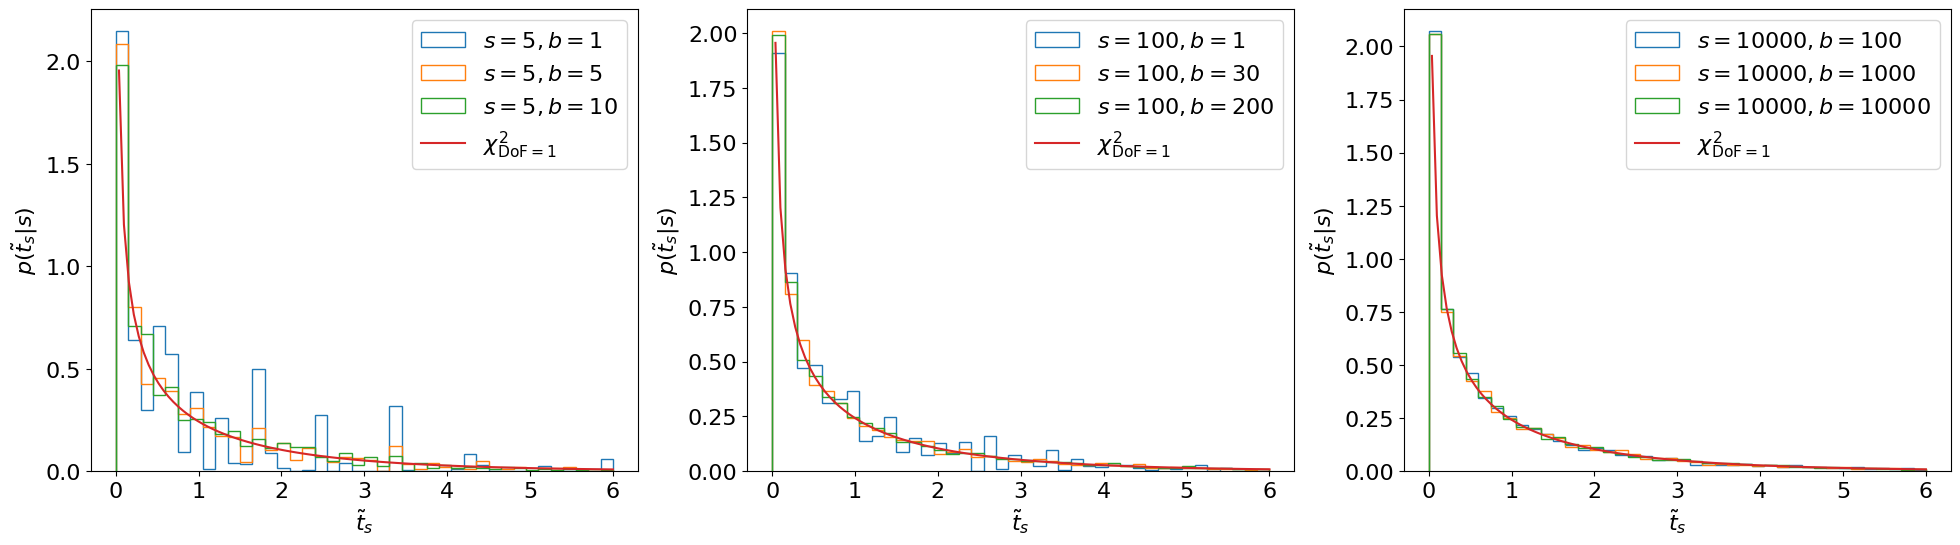
\includegraphics[width=\textwidth]{figures/02-hypothesis-testing/2.png}
\captionsetup{justification=centering}
\caption{Asymptotic form of $p(\tilde{t}_s|s)$.}
\label{fig:p_tilde_t_asym}
\end{figure}

\section{\texorpdfstring{$p$-values}{p-values} and significance}
\label{sec:significance}

Now that we know the distribution of the test statistic $p(\tilde{t}_s|H_s) \equiv p(\tilde{t}_s|s)$, we can finally test $H_s$ with our experiment.
We just need to calculate the ``observed'' test statistic $\tilde{t}^{\mathrm{obs}}_s$ from our observations, and compare it to the $p(\tilde{t}_s|s)$.

\begin{example}
\label{ex:pvalue}
Let's say we're testing the hypothesis of $s = 10$ signal events in our model and we observe $n = 20, m = 5$ events.
We can map this observation to our test statistic $\tilde{{t}}^{\mathrm{{obs}}}_s(s = 10, n_{\mathrm{obs}} = 20, m_{\mathrm{obs}} = 5) = 1.07$,
and see where this falls in our $p(\tilde{t}_s|s)$ distribution (Figure~\ref{fig:Hs}).
\end{example}

\begin{figure}[htb]
\centering
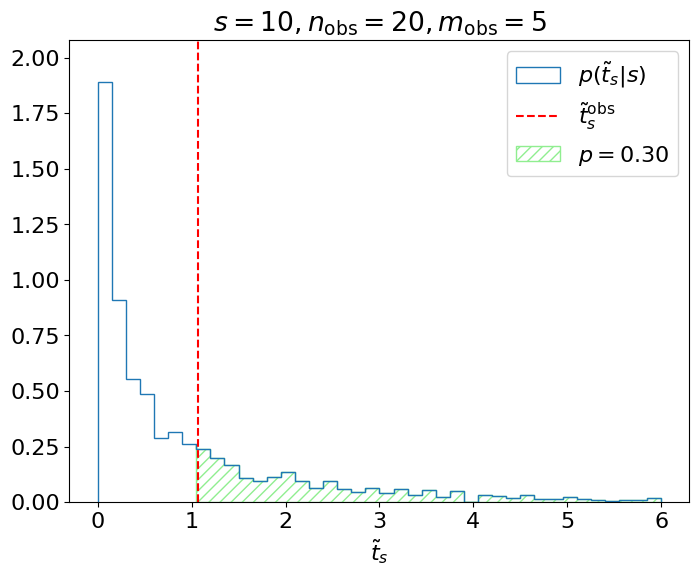
\includegraphics[width=0.6\textwidth]{figures/02-hypothesis-testing/3.png}
\captionsetup{justification=centering}
\caption{Testing $H_s$ in Example~\ref{ex:pvalue}.}
\label{fig:Hs}
\end{figure}

Ultimately, we care about, given $p(\tilde{t}_s|s)$, the probability of obtaining $\tilde{t}^{\mathrm{obs}}_s$ \textit{or a value more inconsistent} with $H_s$; i.e., the green shaded region above.
This is referred to as the $p$\textit{-value} of the observation:
\begin{equation}
p_s = \int_{\tilde{t}_{\mathrm{obs}}}^{\infty}p(\tilde{t}_s|s)\mathrm d \tilde{t}_s = 1 - F(\tilde{t}_{\mathrm{obs}}|s),
\label{eq:pvalue}
\end{equation}
which is $0.30$ for this example, where
\begin{equation}
F(\tilde{t}_s|s) = \int_{-\infty}^{\tilde{t}_s}p(\tilde{t}'_s|s)\mathrm d \tilde{t}'_s
\label{eq:cdf}
\end{equation}
is the cumulative distribution function (CDF) of $\tilde{t}_s$.
We reject the hypothesis if this $p$-value is less than our chosen significance level $\alpha$; the idea being that if $H_s$ were true and we repeated this measurement many times, then the probability of a false-positive ($p$-value $\leq \alpha$) is exactly $\alpha$, as we intended.

The $p$-value is typically converted into a \textit{significance} ($Z$), which is the corresponding number of standard deviations away from the mean in a Gaussian distribution:
\begin{equation}
Z = \Phi^{-1}(1-p),
\label{eq:Z}
\end{equation}
where $\Phi$ is the CDF of the standard Gaussian.
This is more easily illustrated in Figure~\ref{fig:significance}, where $\varphi$ is the standard Gaussian distribution:

\begin{figure}[htb]
\centering
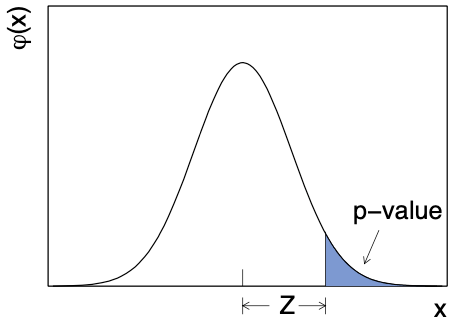
\includegraphics[width=0.6\textwidth]{figures/02-hypothesis-testing/significance.png}
\caption{Relationship between significance $Z$ and the $p$-value, reproduced from Ref.~\cite{Cranmer:2014lly}.}
\label{fig:significance}
\end{figure}

The significance in Example~\ref{ex:pvalue} is, therefore, $\Phi^{-1}(1-0.30) = 0.53$.
We sometimes say that our measurement is (in)consistent or (in)compatible with $H$ at the $0.53\sigma$ level, or within $1\sigma$, etc.

\section{Signal discovery}

So far, we have been testing the signal hypothesis, but usually when searching for a particle, we instead test the ``background-only'' hypothesis $H_0$ and decide whether or not to reject it.
This means we want $\tilde{t}^{\mathrm{obs}}_0$ and $p(\tilde{t}_0|0)$ (Figure~\ref{fig:H0}).\footnote{Ref.~\cite{Cowan:2010js} refers to the special case of the test statistic $\tilde{t}_s$ for $s = 0$ as $q_0$.}

\begin{figure}[htb]
\centering
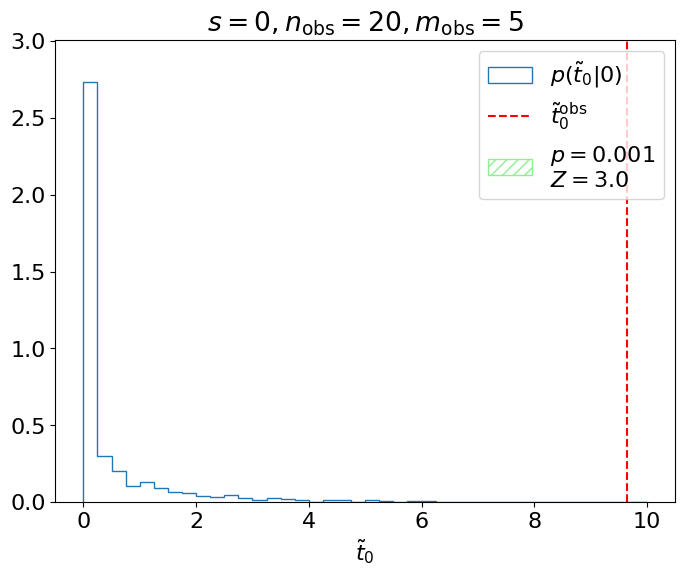
\includegraphics[width=0.6\textwidth]{figures/02-hypothesis-testing/4.png}
\captionsetup{justification=centering}
\caption{Testing the background-only hypothesis in Example~\ref{ex:pvalue}.}
\label{fig:H0}
\end{figure}

We could say for this experiment, therefore, that we exclude the background-only hypothesis at the ``3 sigma'' level.
However, for an actual search for a new particle at the LHC, this is insufficient to claim a discovery, as the probability of a false positive at $3\sigma$, ~1/1000, is too high.
The standard is instead set at $5\sigma$ for discovering new signals, corresponding to the $3\times10^{-7}$ significance level quoted earlier, as we really don't want to be making a mistake if we're claiming to have discovered a new particle!
$3\sigma$, $4\sigma$, and $5\sigma$ are commonly referred to as ``evidence'', ``observation'', and ``discovery'', respectively, of the signals we're searching for.

% \section{Summary}

In summary, the framework for hypothesis testing comprises:

\begin{enumerate}
    \item Defining a test statistic $t$ to map data $\cvec{x}$ (in our example, $\cvec{x} = (n, m)$) to a single number.
    \item Deriving the distribution of $t$ under the hypothesis being tested $p(t|H)$ by sampling from ``toy'' datasets assuming $H$.
    \item Quantifying the compatibility of the observed data $\cvec{x}_{\mathrm{obs}}$ with $H$ with the $p$-value or significance $Z$ of $t_{\mathrm{obs}}$ relative to $p(t|H)$.
\end{enumerate}

This $p$-value / significance is what we then use to decide whether or not to exclude $H$.
A particularly important special case of this, as discussed above, is testing the background-only hypothesis when trying to discover a signal.

\chapter{Confidence intervals and limits}
\label{sec:intervals}

\section{Confidence intervals using the Neyman construction}

Next, we discuss going beyond hypothesis testing to setting intervals and limits for parameters of interest.
The machinery from Section~\ref{sec:hypothesis_testing} can be extended straightforwardly to extracting ``confidence intervals'' for our parameters of interest (POIs): a range of values of the POIs that are allowed, based on the experiment, at a certain ``confidence level'' (CL), e.g. 68\% or 95\%.
Very similar to the idea of the significance level, the CL is defined such that if we were to repeat the experiment many times, a 95\%-confidence-interval must contain, or \textit{cover}, the true value of the parameter 95\% of the time.

This can be ensured for any given CL by solving Eq.~\ref{eq:pvalue} for a $p$-value of $1 - \mathrm{CL}$:
\begin{equation}
p = 1 - \mathrm{CL} = \int_{\tilde{t}^{\mathrm{obs}}_s}^{\infty}p(\tilde{t}_s|s_\pm)\mathrm d \tilde{t}_s,
\label{eq:cl}
\end{equation}
where $s_-$ and $s_+$ are the lower and upper limits on $s$, respectively.

This can be solved by scanning $s$ and finding the values of $s$ for which the RHS $= 1 - \mathrm{CL}$, as demonstrated in Figure~\ref{fig:neymanconstruction} for the experiment in Example~\ref{ex:pvalue} ($n_{\mathrm{obs}} = 20, m_{\mathrm{obs}} = 5$).
This procedure of inverting the hypothesis test by scanning along the values of the POIs is called the ``Neyman construction''.

\begin{figure}[htb]
\centering
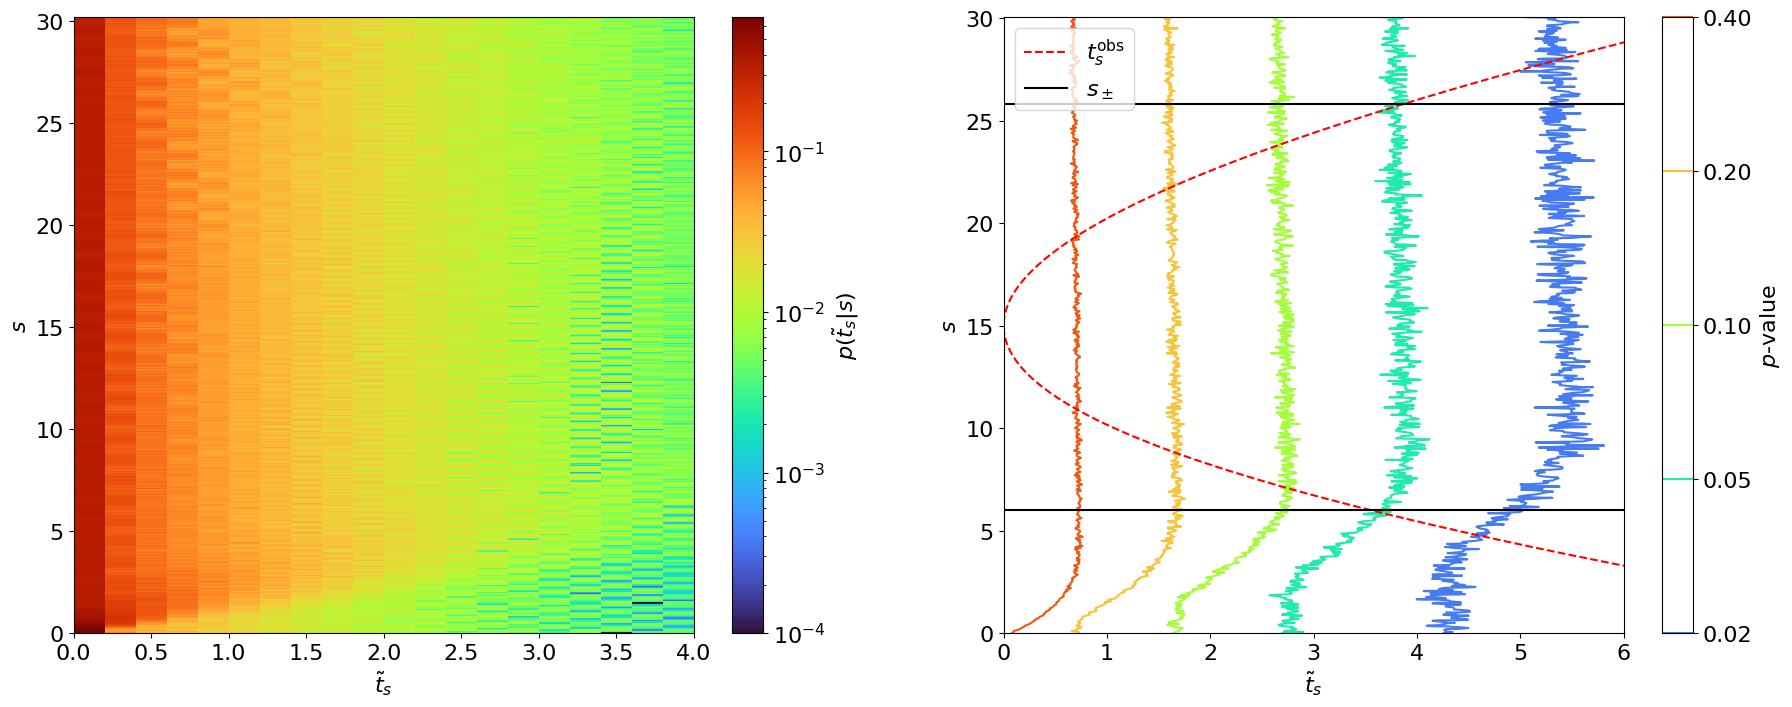
\includegraphics[width=\textwidth]{figures/03-intervals-and-limits/1.png}
\caption[Demonstration of the Neyman construction for a 95\% confidence interval for the experiment in Example~\ref{ex:pvalue} ($n_{\mathrm{obs}} = 20, m_{\mathrm{obs}} = 5$).]{Demonstration of the Neyman construction for a 95\% confidence interval for the experiment in Example~\ref{ex:pvalue} ($n_{\mathrm{obs}} = 20, m_{\mathrm{obs}} = 5$).
Left: Scanning $p(\tilde{t}_s|s)$ using 10,000 toys each for different values of $s$.
Right: Converting this to a contour plot of the $p$-values for different $\tilde{t}_s$'s as a function of $s$, with the observed $t^{\mathrm{obs}}_s$ in red.
The points at which $t^{\mathrm{obs}}_s$ intersects with the $p$-value = 0.05 contour are marked in black and signify the limits of the 95\% confidence interval for $s$ - in this case, $[6.0, 25.8]$.}
\label{fig:neymanconstruction}
\end{figure}

One subtlety to remember is that, in principle, we should also be scanning over the nuisance parameters ($b$) when estimating the $p$-values. However, this would be very computationally expensive so in practice, we continue to use $b = \hat{\hat{b}}(s)$, to always (approximately) maximize the agreement with the hypothesis. Ref.~\cite{Cranmer:2014lly} calls this trick ``profile construction''.

\section{Upper limits}
\label{sec:upper_limits}

Typically if a search does not have enough sensitivity to directly observe a new signal, we instead quote an upper limit on the signal strength.
This is similar in practice to the Neyman construction for confidence intervals, solving Eq.~\ref{eq:cl} only for the upper boundary. However, an important difference is that when setting upper limits, we have to modify the test statistic so that a best-fit signal strength \textit{greater} than the expected signal ($\hat{s} > s$) does not lower the compatibility with $H_s$:
\begin{gather}
    \tilde{q}(s) = \left\{
        \begin{array}{ll}
          \tilde{t}(s), & \mbox{$\hat{s} < s$}.\\
          0, & \mbox{$\hat{s} \geq s$}.
        \end{array}
      \right.
      = \left\{
        \begin{array}{ll}
          -2\ln\tilde{\lambda}(s), & \mbox{$\hat{s} < s$}.\\
          0, & \mbox{$\hat{s} \geq s$}.
        \end{array}
      \right.
      = \left\{
      \begin{array}{ll}
          -2\ln\frac{L(s, \hat{\hat{b}}(s))}{L(0, \hat{\hat{b}}(0))}, & \mbox{$\hat{s}<0$}.\\
          -2\ln\frac{L(s, \hat{\hat{b}}(s))}{L(\hat{s}, \hat{b})}, & \mbox{0 $\leq \hat{s} < s$}.\\
          0, & \mbox{$\hat{s} \geq s$}.
        \end{array}
      \right.
  \label{eq:qs_tilde}
\end{gather}

The upper limit test statistic $\tilde{q}(s)$ is set to $0$ for $\hat{s} > s$ so that this situation does not contribute to the $p$-value integral in Eq.~\ref{eq:pvalue}.
Figure~\ref{fig:q_tilde_s} demonstrates this, and the difference between $\tilde{t}_s$ and $\tilde{q}_s$, for different sample observations.

\begin{figure}[htb]
\centering
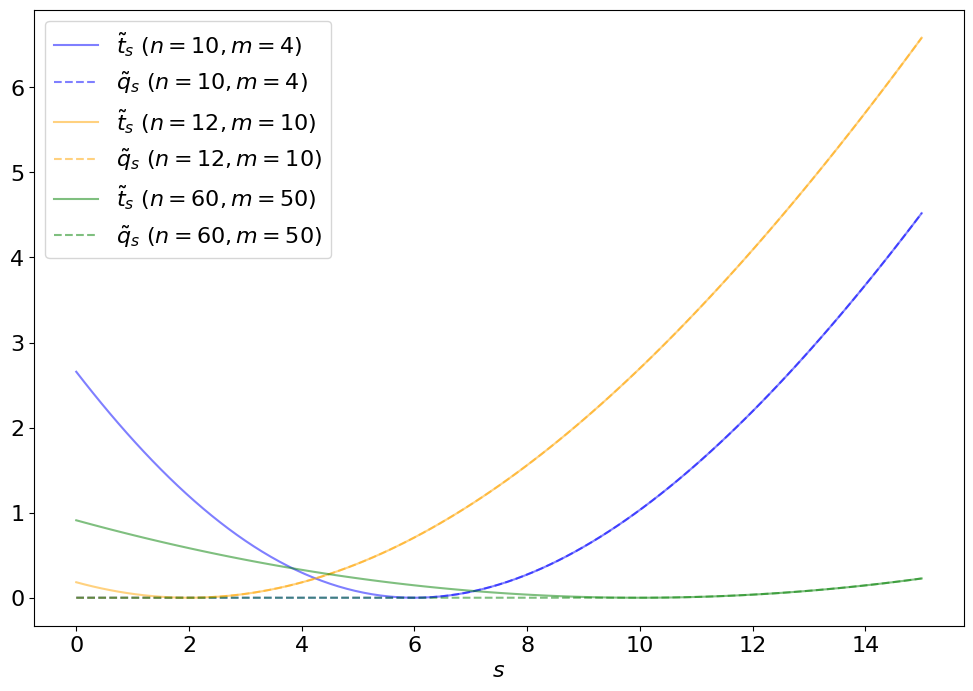
\includegraphics[width=0.7\textwidth]{figures/03-intervals-and-limits/2.png}
\captionsetup{justification=centering}
\caption{Comparing $\tilde{t}_s$ and $\tilde{q}_s$.}
\label{fig:q_tilde_s}
\end{figure}

Note that (as one may expect from Figure~\ref{fig:q_tilde_s}) the distribution $p(\tilde{q}_s|s)$ no longer behaves like a standard $\chi^2$ but, instead, as a ``half-$\chi^2$''.
This is essentially a $\chi^2$ plus a delta function at 0 (since, under the signal hypothesis, on average there will be an over-fluctuation half the time, for which $\tilde{q}_s = 0$), as shown in Figure~\ref{fig:p_tilde_q}.

\begin{figure}[htb]
\centering
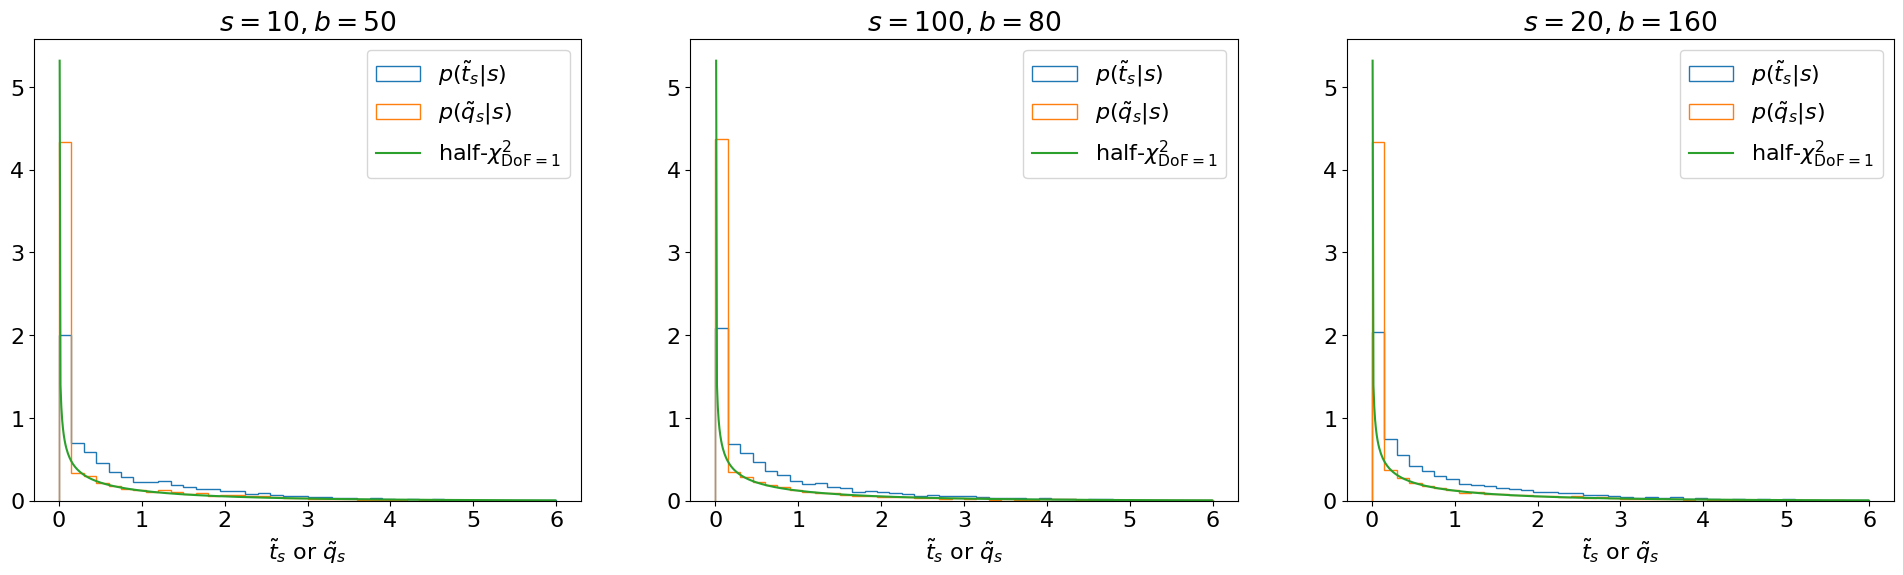
\includegraphics[width=\textwidth]{figures/03-intervals-and-limits/3.png}
\caption{Comparing $p(\tilde{t}_s|s)$ and $p(\tilde{q}_s|s)$. $p(\tilde{q}_s|s)$ asymptotically follows a half-$\chi^2$ distribution (green).}
\label{fig:p_tilde_q}
\end{figure}

We can now revisit Example~\ref{ex:pvalue} to set an upper limit on $s$ rather than a confidence interval (Figure~\ref{fig:upperlimits}).
$p(\tilde{q}_s|s)$ is shifted to the left with respect to $p(\tilde{t}_s|s)$; hence, the upper limit of $24$ is slightly lower than the upper bound of the 95\% confidence interval we derived using $\tilde{t}_s$.

\begin{figure}[htb]
\centering
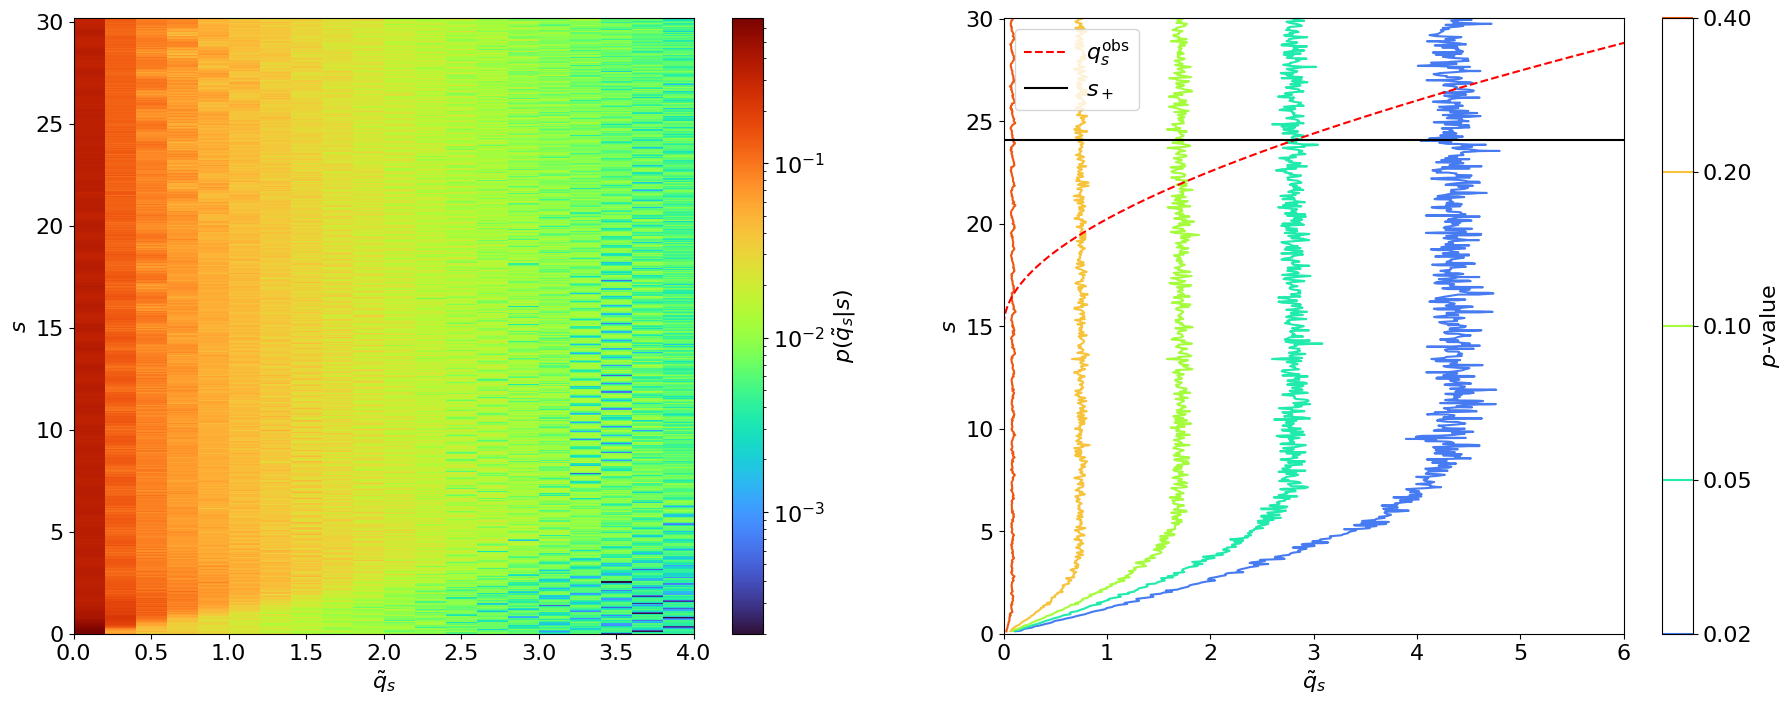
\includegraphics[width=\textwidth]{figures/03-intervals-and-limits/4.png}
\caption[Extending the Neyman construction to an upper limit on $s$.]{Extending the Neyman construction to an upper limit on $s$.
Left: Scanning the upper limit test statistic distribution $p(\tilde{q}_s|s)$ using 10,000 toys each for different values of $s$.
Right: Converting this to a contour plot of the $p$-values for different $\tilde{q}_s$'s as a function of $s$, with the observed $q^{\mathrm{obs}}_s$ in red.
The point at which $q^{\mathrm{obs}}_s$ intersects with the $p$-value = 0.05 contour is marked in black and signifies the upper limit at 95\% CL.}
\label{fig:upperlimits}
\end{figure}

\section{The \texorpdfstring{CL$_s$}{CLs} criterion}
\label{sec:cls}

We now introduce two conventions related to hypothesis testing and searches in particle physics.
Firstly (the simple one), the POI $s$ is usually re-parametrized as $s \rightarrow \mu \cdot s$,
where $\mu$ is now considered the POI, referred to as the ``signal strength'', and $s$ is a fixed value representing the number of signal events we expect to see for the nominal signal strength $\mu$ of $1$.
For the example in Figure~\ref{fig:upperlimits}, if we expect $s = 10$ signal events, then we would quote the upper limit as $24 / s = 2.4$ on $\mu$ at 95\% CL.

The second, important, convention is that we use a slightly different criterion for confidence intervals, called ``CL$_s$''.
This is motivated by situations where we have little sensitivity to the signal we're searching for, as in the below example.

\begin{example}
\label{ex:cls}
Let's say we expect $s = 10$ and observe $n = 70$, $m = 100$.
Really, what this should indicate is that our search is not at all sensitive, since our search region is completely dominated by background and, hence, we should not draw strong conclusions about the signal strength.
However, if we follow the above procedure for calculating the upper limit, we get $\mu \leq 0.001$ at 95\% CL.
\end{example}

This is an extremely aggressive limit on $\mu$, where we're excluding the nominal $\mu = 1$ signal at a high confidence level.
Given the complete lack of sensitivity to the signal, this is not a sensible result.
The CL$_s$ method solves this problem by considering both the $p$-value of the signal + background hypothesis $H_s$ (referred to as $p_{s+b}$ or just $p_\mu$ for short), \textit{and} the $p$-value of the background-only hypothesis $H_0$ ($p_b$), to define a new criterion:
\begin{equation}
p_\mu' = \frac{p_\mu}{1 - p_b}
\label{eq:pmu_prime}
\end{equation}

In cases where the signal region is completely background-dominated, the compatibility with the background-only hypothesis should be high, so $p_b \sim 1$ and, hence, $p_\mu'$ will be increased.
On the other hand, for more sensitive regions, compatibility should be lower $\Rightarrow p_b \sim 0$ and $p_\mu' \sim p_\mu$.

To be explicit, here
\begin{equation}
p_b = \int^{\tilde{t}_{\mathrm{obs}}}_{-\infty}p(\tilde{t}_s|0)\mathrm d \tilde{t}_s,
\label{eq:pb}
\end{equation}

where we should note that:
\begin{enumerate}
    \item We're looking at the distribution of $\tilde{t}_s$ --- \textit{not} $\tilde{t}_0$ --- under the background-only hypothesis, since the underlying test is of $H_s$, not $H_0$; and
    \item We're integrating \textit{up to} $\tilde{t}_{\mathrm{obs}}$, unlike for $p_s$, because lower $\tilde{t}$ means greater compatibility with the background-only hypothesis.
\end{enumerate}

The effect of the CL$_s$ criterion is demonstrated in Figure~\ref{fig:cls} for Examples~\ref{ex:pvalue} and~\ref{ex:cls}.
In the former, the background-only distribution is shifted to the right of the $s+b$ distribution.
This indicates that the experiment is sensitive to $\mu$ and, indeed, we find $p_\mu' \sim p_\mu$.
In Example~\ref{ex:cls}, however, the search is not sensitive and, hence, the background-only and $s+b$ distributions almost completely overlap, meaning $p_b \sim 1$ and $p_\mu' >> p_\mu$.\footnote{Note that, unlike $p(\tilde{t}_s|s)$, $p(\tilde{t}_s|0)$ \textit{doesn't} follow a simple $\chi^2$; asymptotically, it is closer to a \textit{noncentral} $\chi^2$, as will be discussed in Section~\ref{sec:asymptotic_plr}.
}

\begin{figure}[htb]
\centering
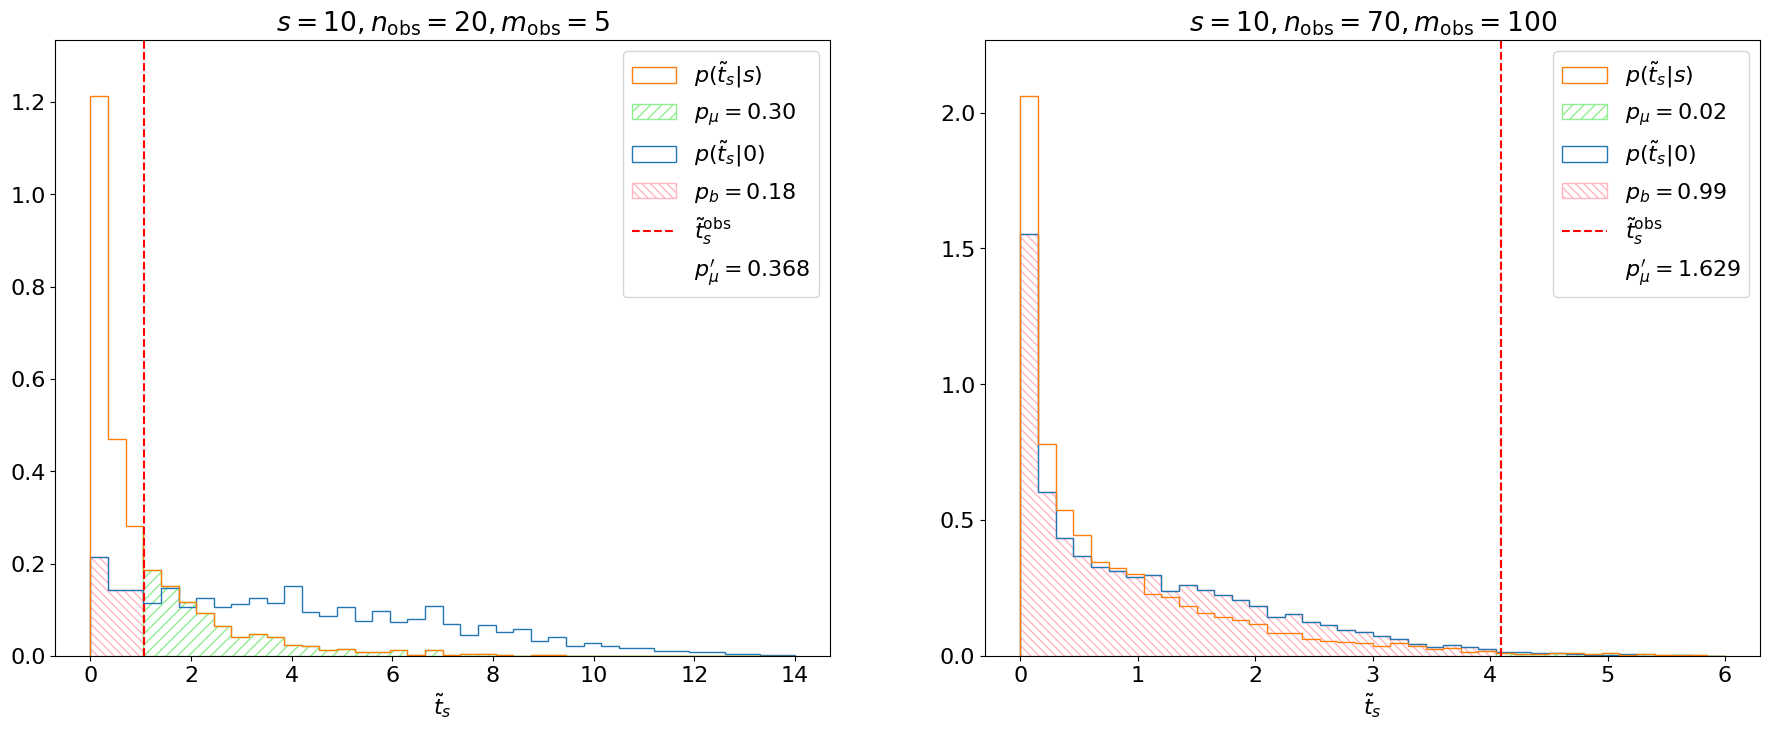
\includegraphics[width=\textwidth]{figures/03-intervals-and-limits/5.png}
\captionsetup{justification=centering}
\caption{Demonstration of CL$_s$ criterion for Examples~\ref{ex:pvalue} (left) and~\ref{ex:cls} (right).}
\label{fig:cls}
\end{figure}

Finally, if we repeat the Neyman construction using the CL$_s$ criterion $p_\mu'$ instead of $p_\mu$ for Example~\ref{ex:cls}, we can find an upper limit of $\mu \leq 1.2$ at 95\% CL, which is indeed a looser, more conservative, upper limit.
The upper limit for Example~\ref{ex:pvalue} remains unchanged at $\mu \leq 2.4$, as we would expect.


\chapter{Expected significances and limits}
\label{sec:expected}

\section{Expected significance}

The focus so far has been only on evaluating the \textit{results} of experiments.
However, it is equally important to characterize the expected sensitivity of the experiment \textit{before} running it (or before looking at the data).

\begin{example}
\label{ex:expsig}
Concretely, we continue with the simple one-bin counting experiment (Section~\ref{sec:data_model}).
Let's say we expect $b = 10$ background events and --- at the nominal signal strength $\mu = 1$ --- $s = 10$ signal events.
How do we tell if this experiment is at all useful for discovering this signal, i.e., does it have any sensitivity to the signal?
\end{example}

One way is to calculate the significance with which we expect to exclude the background-only hypothesis if the signal were, in fact, to exist.
Practically, this means we are testing $H_0$ and, hence, need $p(\tilde{t}_0|\mu = 0)$ as before. However, now we also need the distribution of the test statistic $\tilde{t}_0$ under the \textit{background + signal} hypothesis $p(\tilde{t}_0|\mu = 1)$.
Then, by calculating the significance for each sampled $\tilde{t}_0$ under $H_{\mu = 1}$, we can estimate the distribution of expected significances.
This is illustrated for Example~\ref{ex:expsig} in Figure~\ref{fig:expZ}.

\begin{figure}[htb]
\centering
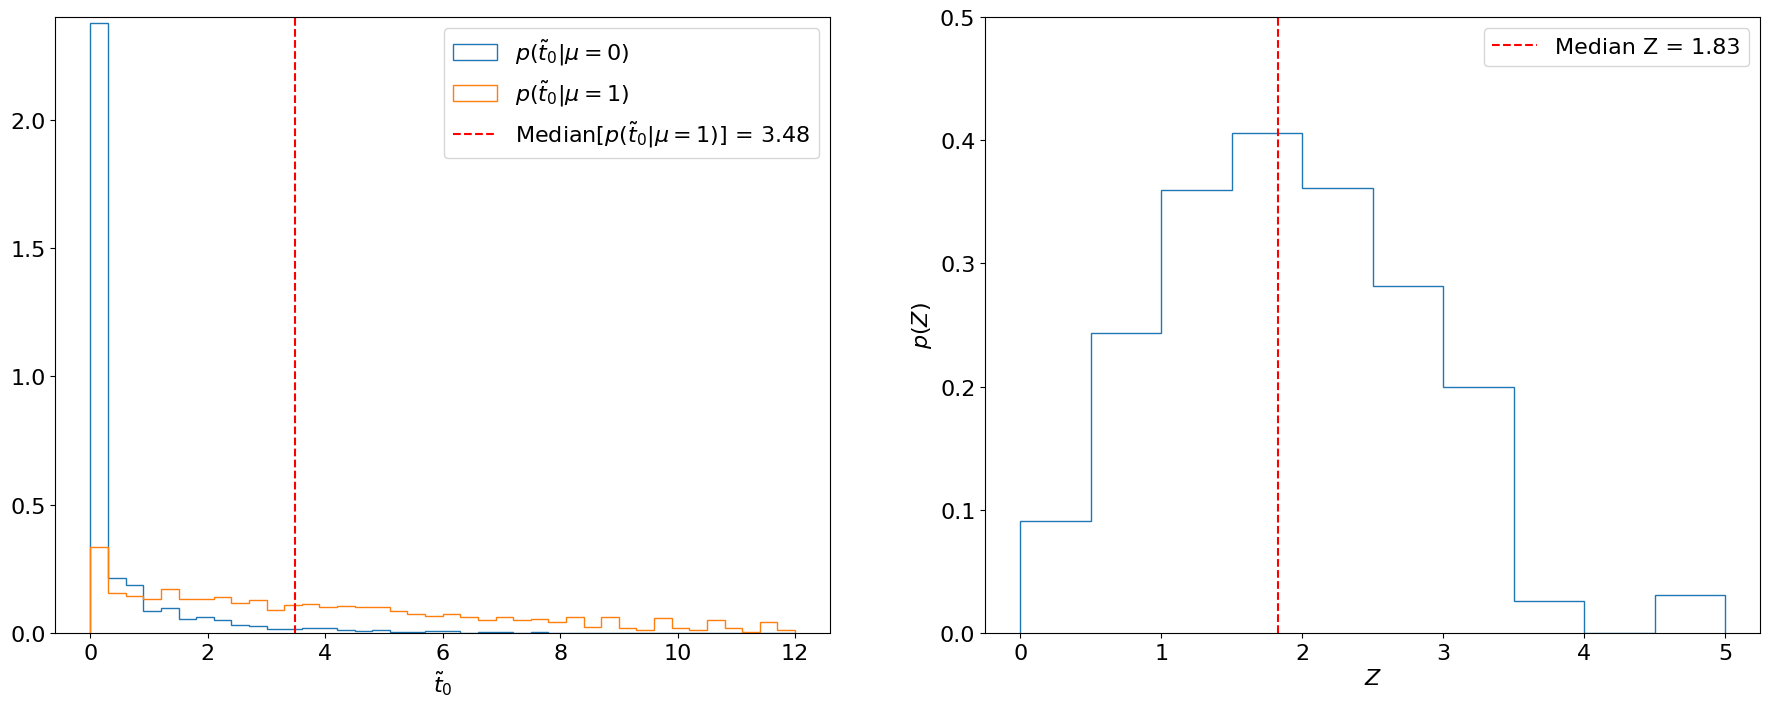
\includegraphics[width=\textwidth]{figures/04-expected/1.png}
\caption[Left: Distributions of $\tilde{t}_0$ under the background-only and background + signal hypotheses using 30,000 toys each.]{Left: Distributions of $\tilde{t}_0$ under the background-only and background + signal hypotheses using 30,000 toys each.
The median of the latter is marked in red.
Right: Distribution of the significances (with respect to the background-only hypothesis) of each sampled $\tilde{t}_0$ under the signal hypothesis.
}
\label{fig:expZ}
\end{figure}

Importantly, we usually quote the \textbf{median} of this distribution as the expected significance, since the median is ``invariant'' to monotonic transformations (i.e., the median $p$-value will always correspond to the median $Z$ as well, whereas the mean $p$-value will not correspond to the mean $Z$).
Similarly, we quote the $16\%/84\%$ and $2\%/98\%$ quantiles as the $\pm 1\sigma$ and $\pm 2\sigma$, respectively, expected significances.
These quantiles correspond to the cumulative probabilities for a standard Gaussian (Figure~\ref{fig:gaussian_quantiles}).
For Example~\ref{ex:expsig}, we thus find the median expected significance to be 1.83.

\begin{figure}[htb]
\centering
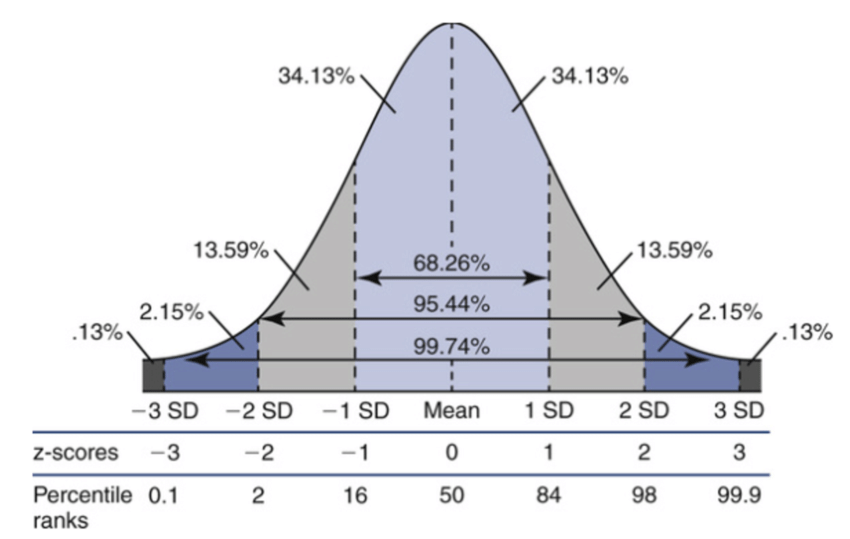
\includegraphics[width=0.6\textwidth]{figures/04-expected/gaussian_quantiles.png}
\captionsetup{justification=centering}
\caption{Gaussian quantiles, reproduced from Ref.~\cite{Stiller:thesis}.}
\label{fig:gaussian_quantiles}
\end{figure}

Note that instead of converting each sampled $\tilde{t}$ under $H_{\mu=1}$ into a significance and finding the median of that distribution, as in Figure~\ref{fig:expZ} (right), we can take advantage of the invariance of the median and directly use the significance of the median $\tilde{t}$ under $H_{\mu=1}$ (Figure~\ref{fig:expZ}, left).
We will do this below for the expected limit.

\section{Expected limits}

The other figure of merit we care about in searches is the upper exclusion limit set on the signal strength.
To derive the \textit{expected} limit, we do the opposite of the above and ask, if the signal were not to exist, what value of $\mu$ would we expect to exclude at the 95\% CL.\footnote{$95\%$ is the standard CL for upper limits in HEP.}

This means we need:
\begin{enumerate}
  \item The distribution $p(\tilde{q}_\mu|\mu)$ to solve for $\mu^+$ in Eq.~\ref{eq:cl} and be able to do the upper limit calculation (as in Section~\ref{sec:upper_limits});
  \item $p(\tilde{q}_\mu|0)$ to get the median (and other quantiles') expected $\tilde{q}_\mu^{\mathrm{obs}}$ for different signal strengths under the background-only hypothesis; and, furthermore,
  \item To scan over the different signal strengths to find the $\mu$ that results in a median $p$-value of $0.05$ --- or, rather, $p_\mu'$-value (Eq.~\ref{eq:pmu_prime}), since we're using the CL$_s$ method for upper limits (Section~\ref{sec:cls}).
\end{enumerate}

First, let's look at the first two steps for just the $\mu = 1$ signal strength in Example~\ref{ex:expsig}.
These steps are similar to, and essentially an inversion of, the procedure for the expected significance: we're now finding the $p_{\mu=1}'$-value with respect to the signal + background hypothesis, for the median $\tilde{q}_\mu$ sampled under the background-only hypothesis.
This is demonstrated in Figure~\ref{fig:explim}.

\begin{figure}[htb]
\centering
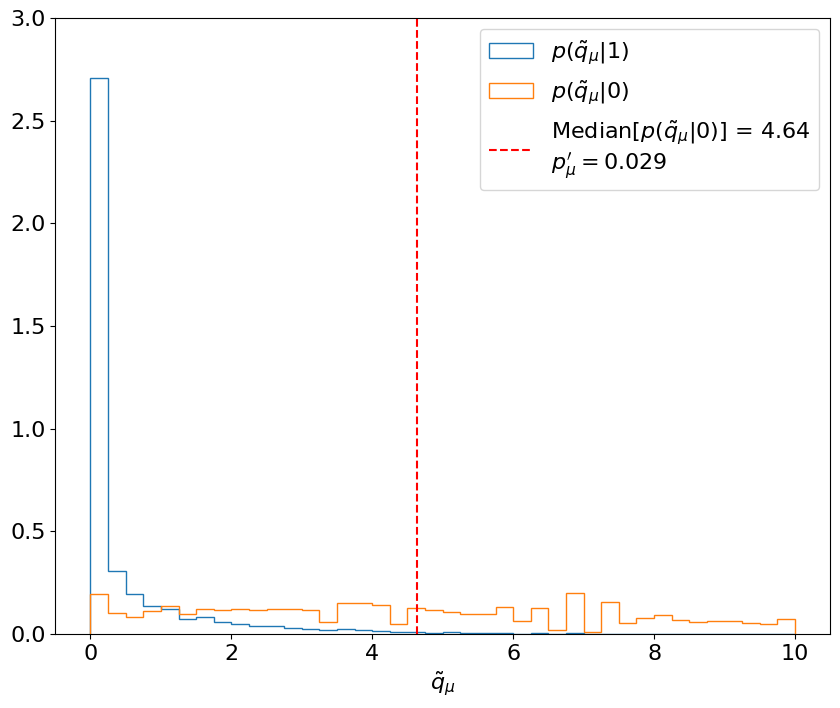
\includegraphics[width=0.7\textwidth]{figures/04-expected/2.png}
\caption[Calculating the median expected $p_{\mu=1}'$-value with respect to the signal + background hypothesis, for test statistics $\tilde{q}_\mu$ sampled under the background-only hypothesis.]{Calculating the median expected $p_{\mu=1}'$-value with respect to the signal + background hypothesis, for test statistics $\tilde{q}_\mu$ sampled under the background-only hypothesis.
$p(\tilde{q}_\mu|1)$ and $p(\tilde{q}_\mu|0)$ are estimated using 30,000 toys each.
Then, the median $p(\tilde{q}_\mu|0)$ (red) is used to calculate the $p_{\mu}'$-value following the CL$_s$ criterion.}
\label{fig:explim}
\end{figure}

The key difference with respect to calculating the expected significance is step 3, in which this procedure has to be repeated for a range of signal strengths to find the value that gives a median (and $\pm1\sigma,\pm2\sigma$ quantile-) $p_\mu'$ of $0.05$.
This is thus the minimum value of $\mu$ that we expect to be able to exclude at 95\% CL, as shown in Figure~\ref{fig:explim2}.

\begin{figure}[htb]
\centering
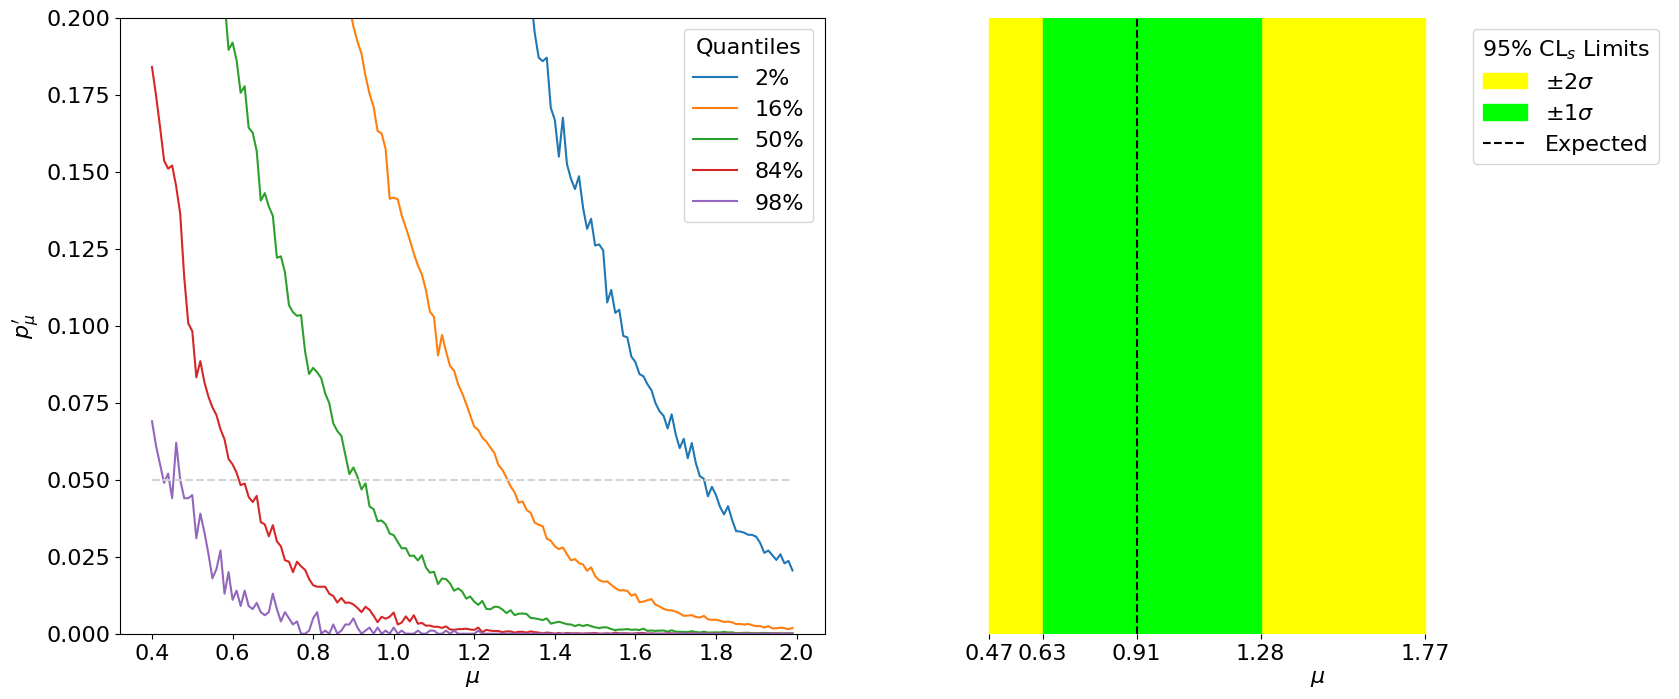
\includegraphics[width=\textwidth]{figures/04-expected/3.png}
\caption{Left: The expected median and $\pm1\sigma,\pm2\sigma$ quantiles of $p_\mu'$ for different $\mu$'s. The intersection of these with $p_\mu' = 0.05$ (gray) corresponds to the expected exclusion limits. Right: The median and $\pm 1\sigma, \pm 2\sigma$ expected limits at 95\% CL$_s$ on $\mu$.}
\label{fig:explim2}
\end{figure}


Thus, we have our expected limits.
The right plot of Figure~\ref{fig:explim2} is colloquially known as a ``Brazil-band plot'', and is the standard way of representing limits.
For example, Figure~\ref{fig:atlas_higgs} is the corresponding plot by ATLAS for the Higgs discovery (scanning over the Higgs mass).

\begin{figure}[htb]
\centering
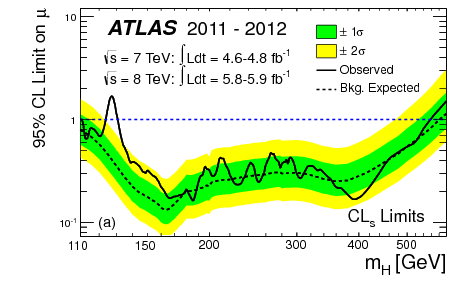
\includegraphics[width=0.6\textwidth]{figures/04-expected/atlas_limits.png}
\caption{Expected and observed 95\% CL$_s$ upper limits for the SM Higgs by ATLAS in 2012, for different hypothetical Higgs masses~\cite{ATLAS:2012yve}.}
\label{fig:atlas_higgs}
\end{figure}


\part{Asymptotic formulae}
\label{sec:asymptotic}

\chapter{Asymptotic form of the MLE}
\label{sec:asymptotic_mle}

So far, we have discussed how to extract meaningful statistical results from HEP experiments by making extensive use of pseudodata / toy experiments to estimate the sampling distributions of profile-likelihood-ratio-based test statistics.
While this worked nicely for our simple counting experiment, generating a sufficiently large number of toys can quickly become computationally intractable for the more complex searches (and statistical combinations of searches) that are increasingly prevalent at the LHC, containing at times up to thousands of bins and nuisance parameters.
This and the following section discuss a way to approximate these sampling distributions without the need for pseudodata.
This was introduced in the famous ``CCGV'' paper~\cite{Cowan:2010js} in 2011 and has since become the de-facto procedure at the LHC.

As hinted at previously, such as in Figures~\ref{fig:p_tilde_t_asym} and~\ref{fig:p_tilde_q}, the distributions $p(\tilde{t}_\mu|\mu')$ and $p(\tilde{q}_\mu|\mu')$ (where, in general, $\mu' \neq \mu$) have similar forms regardless of the nuisance parameters (or sometimes even the POIs).
This is not a coincidence: we will now derive their ``asymptotic'' --- i.e., in the large sample limit --- forms, starting first with the asymptotic form of the maximum likelihood estimator (MLE).

It is important to remember that the MLE $\hat \mu$ of $\mu$ is a random variable with its own probability distribution.
We can estimate it as always by sampling toys, shown in Figure~\ref{fig:p_mle} for our counting experiment (Eq.~\ref{eq:pois3}).
One can observe that $p(\hat \mu)$ follows a Gaussian distribution as the number of events $N$ increases, and indeed this becomes clear if we try to fit one to the histograms (Figure~\ref{fig:p_mle_fit}).
We will now show this to be true generally, deriving the analytic distribution in Sections~\ref{sec:pmle_bg}---\ref{sec:pmle_derivation}, and discussing the results and the important concept of the \textit{Asimov} dataset for numerical estimation in Sections~\ref{sec:pmle_result} and~\ref{sec:pmle_asimov}, respectively.

\begin{figure}[htb]
\centering
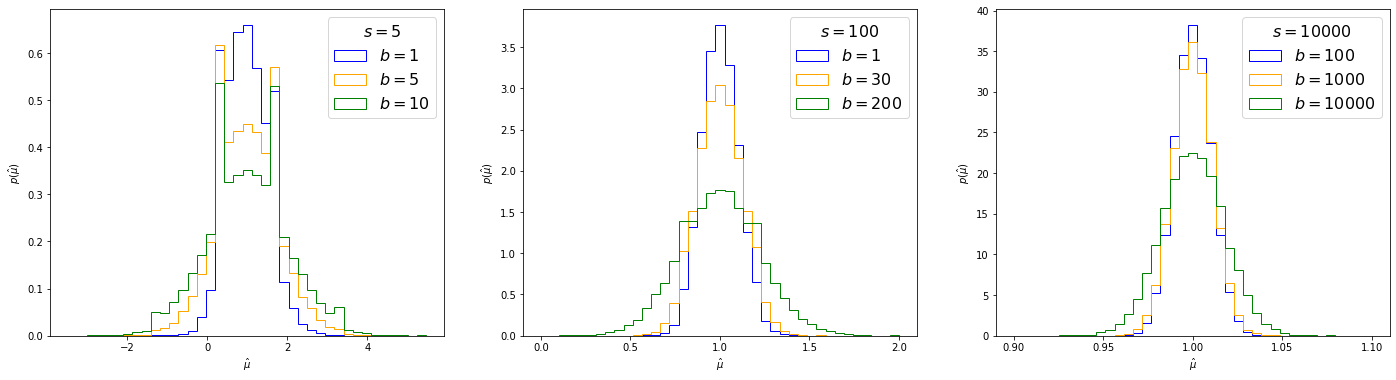
\includegraphics[width=\textwidth]{figures/05-asymptotic-mle/1.png}
\caption{Distribution of the MLE of $\mu$ for different $s$ and $b$ produced using 30,000 toy experiments each. (Note the x-axis range is becoming narrower from the left-most to the right-most plot.)}
\label{fig:p_mle}
\end{figure}

\begin{figure}[htb]
\centering
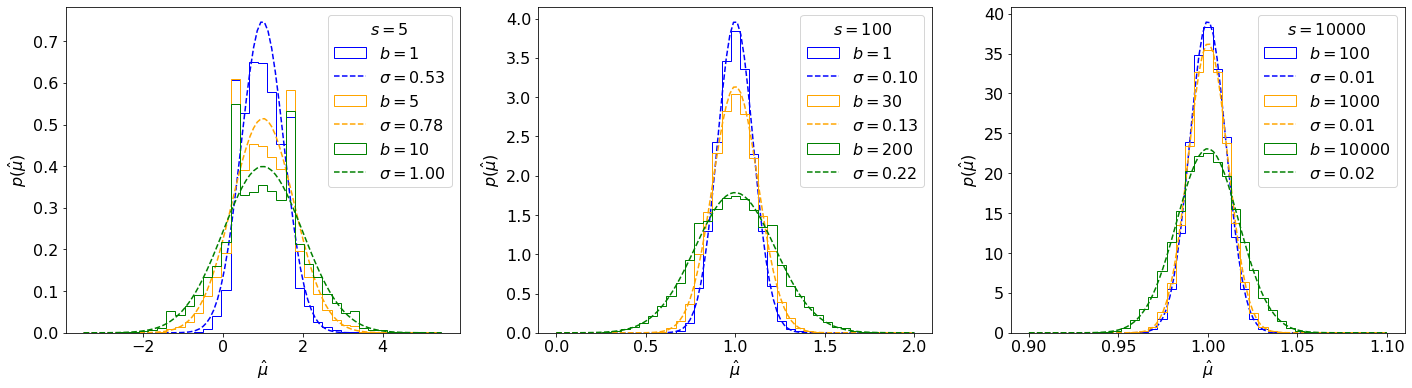
\includegraphics[width=\textwidth]{figures/05-asymptotic-mle/2.png}
\caption{Gaussian fits to distributions of $\hat\mu$ for different $s$ and $b$ from Figure~\ref{fig:p_mle}.}
\label{fig:p_mle_fit}
\end{figure}


\section{Statistics background}
\label{sec:pmle_bg}

We first provide a lightning review of some necessary statistics concepts and results.

\begin{definition}
\label{def:score}
Let the negative log-likelihood (NLL) $-\ln L(\mu) \equiv -l(\mu)$.
The derivative of the NLL $-l'(\mu)$ is called the \textbf{score} $s(\mu)$.
It has a number of useful properties:
\footnote{See derivations in e.g. Ref.~\cite{enwiki:1253018821}.}
\begin{enumerate}
  \item Its expectation value at $\mu'$ $\mathbb E_{\mu = \mu'}[s(\mu')] = 0$.
  \item Its variance $\mathrm {Var} [s(\mu)] = - \mathbb E [l''(\mu)]$.
\end{enumerate}
Note that the expectation value here means an average over observations which are distributed according to a particular $\mu$, which here we're calling the ``true'' $\mu$: $\mu'$.
\end{definition}

\begin{definition}
\label{def:fisher_information}
$- \mathbb E [l''(\mu)] \equiv \mathcal I(\mu)$ is called the \textbf{Fisher information}.
It quantifies the information our data contains about $\mu$ and importantly, as we'll see, it (approximately) represents the inverse of the variance of $\hat \mu$.
More generally, for multiple parameters,
\begin{equation}
\label{eq:fisher_matrix}
\mathcal I_{ij}(\mu) = - \mathbb E [\frac{\partial^2 l}{\partial \mu_i \partial \mu_j}]
\end{equation}
is the Fisher information matrix.
It is also commonly called the \textbf{covariance matrix}.
\end{definition}

\begin{theorem}
Putting this together, by the central limit theorem~\cite{enwiki:1257009135}, this means $p(s(\mu'))$ follows a normal distribution with mean $0$ and variance $\mathcal I(\mu')$, up to terms of order $\mathcal O(\frac{1}{\sqrt{N}})$:
\begin{equation}
s(\mu') \xrightarrow{\sqrt{N} >> 1} \mathcal N(0, \sqrt{\mathcal I(\mu')}),
\label{eq:score}
\end{equation}
where $N$ represents the data sample size.
\end{theorem}


\section{The Fisher information}

For our simple counting experiment, the Fisher information matrix $\mathcal I(\mu, b)$ can be found by taking second derivatives of the NLL (Eq.~\ref{eq:nll}).
The $\mathcal I_{\mu\mu}$ term, for example, is:
\begin{equation}
    \mathcal I_{\mu\mu}(\mu, b) = - \mathbb E[\partial^\mu\partial^\mu l(\mu, b)] = \mathbb E \bigg[n \cdot \frac{s^2}{(\mu s + b)^2}\bigg] = \mathbb E[n] \cdot \frac{s^2}{(\mu s + b)^2} = \frac{(\mu' s + b') s^2}{(\mu s + b)^2}.
\label{eq:fisher}
\end{equation}

In the last step we use the fact that $\mathbb E[n]$ under true $\mu = \mu'$, $b = b'$, is $\mu' s + b'$.
For the remainder of this section, $\mathcal I(\mu, b)$ will always be evaluated at the true values of the parameters,\footnote{The reason for this is discussed shortly in Section~\ref{sec:pmle_derivation}.} so this can be simplified to $\mathcal I_{\mu\mu}(\mu', b') = \frac{s^2}{\mu' s + b'}$.
This is plotted in Figure~\ref{fig:fisher}, where we can the Fisher information captures the fact that as $b$ increases, we lose sensitivity to --- or \textit{information} about --- $\mu$.

\begin{figure}[htb]
\centering
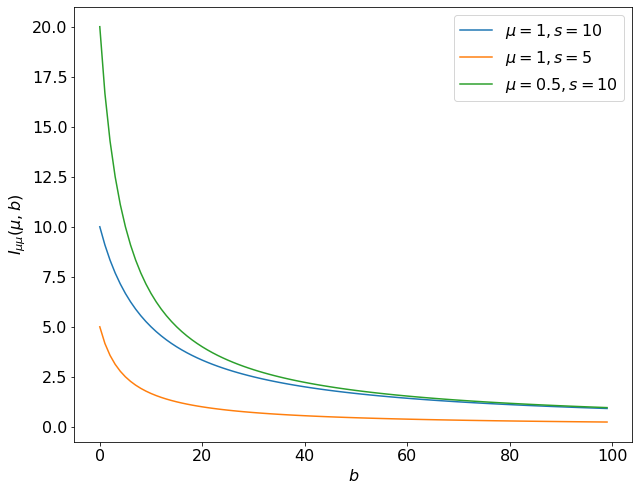
\includegraphics[width=0.7\textwidth]{figures/05-asymptotic-mle/3.png}
\caption{The Fisher information $\mathcal I_{\mu\mu}(\mu, b)$ for different $\mu$ and $s$, as a function of the expected background $b$.}
\label{fig:fisher}
\end{figure}

For completeness (and since we'll need it below), the full Fisher information matrix for our problem, repeating the steps in Eq.~\ref{eq:fisher}, is:
\begin{equation}
    \mathcal I(\mu', b')
    = \begin{pmatrix}\mathcal I_{\mu\mu} & \mathcal I_{\mu b} \\ \mathcal I_{b\mu} & \mathcal I_{bb}\end{pmatrix}(\mu', b')
    = \begin{pmatrix}
    \frac{s^2}{\mu' s + b'} & \frac{s}{\mu' s + b'} \\ \frac{s}{\mu' s + b'} & \frac{1}{\mu' s + b'} + \frac{1}{b'}
    \end{pmatrix}
\label{eq:fishermatrix}
\end{equation}


\section{Derivation}
\label{sec:pmle_derivation}

We now have enough background to derive the asymptotic form of the MLE.
We do this for the 1D case by Taylor-expanding the score of $\hat \mu$, $l'(\hat\mu)$ - which we know to be $ = 0$ - around $\mu'$:
\begin{align}
l'(\hat\mu) &= l'(\mu') + l''(\mu')(\hat\mu - \mu') + \mathcal O((\hat\mu - \mu')^2) = 0 \\
\Rightarrow \hat\mu - \mu' &\simeq - \frac{l'(\mu')}{l''(\mu')} \xrightarrow{\sqrt{N} >> 1} \frac{1}{\mathcal I(\mu')}N(0, \sqrt{\mathcal I(\mu')}) = N\bigg(0, \frac{1}{\sqrt{\mathcal I(\mu')}}\bigg),
\label{eq:taylorl}
\end{align}

where we plugged in the distribution of $l'(\mu')$ from Eq.~\ref{eq:score}, claimed $l''(\mu')$ asymptotically equals its expectation value $\mathbb E[l''(\mu')] = \mathcal I(\mu')$ by the law of large numbers~\cite{enwiki:1256071749}, and are ignoring the $\mathcal O((\hat\mu - \mu')^2)$ term.\footnote{For a more rigorous derivation, see e.g. Ref.~\cite{gundersen_asymptotic_2019}.}

For multiple parameters, $\mathcal I$ is a matrix so the variance generalized to the matrix inverse:
\begin{equation}
    \hat\mu - \mu' \simeq N(0, \sqrt{\mathcal I^{-1}_{\mu\mu}(\mu', b')}),
\label{eq:asym_std_fisher}
\end{equation}

\section{Result}
\label{sec:pmle_result}

Thus, we see that $\hat \mu$ asymptotically follows a normal distribution around the true $\mu$ value, $\mu'$, with a variance $\sigma_{\hat\mu}^2 = \mathcal I^{-1}_{\mu\mu}(\mu', b')$, up to $\mathcal O (1/\sqrt{N})$ terms.
Intuitively, from the definition of the Fisher information $\mathcal I$, we can interpret this as saying that the more information we have about $\mu$ from the data, the lower the variance should be on $\hat \mu$.

Continuing with our counting experiment from Section~\ref{sec:data_model}, inverting $\mathcal I$ from Eq.~\ref{eq:fishermatrix} gives us
\begin{equation}
    \sigma_{\hat\mu} = \sqrt{\mathcal I^{-1}_{\mu\mu}(\mu', b')} = \frac{\sqrt{\mu' s + 2b'}}{s}.
\label{eq:asymstd}
\end{equation}

Note that, as we might expect, this scales as $\sim \sqrt{b}$, which is the uncertainty of our Poisson nuisance parameter $b$ --- showing mathematically why we want to keep uncertainties on nuisance parameters as low as possible.
This is compared to the toy-based distributions from Section~\ref{sec:asymptotic_mle} in Figure~\ref{fig:p_mle_asym} this time varying the true signal strength $\mu'$ as well, where we can observe that this matches very well for large $s, b$, while for small values there are some discrete differences.

\begin{figure}[htb]
\centering
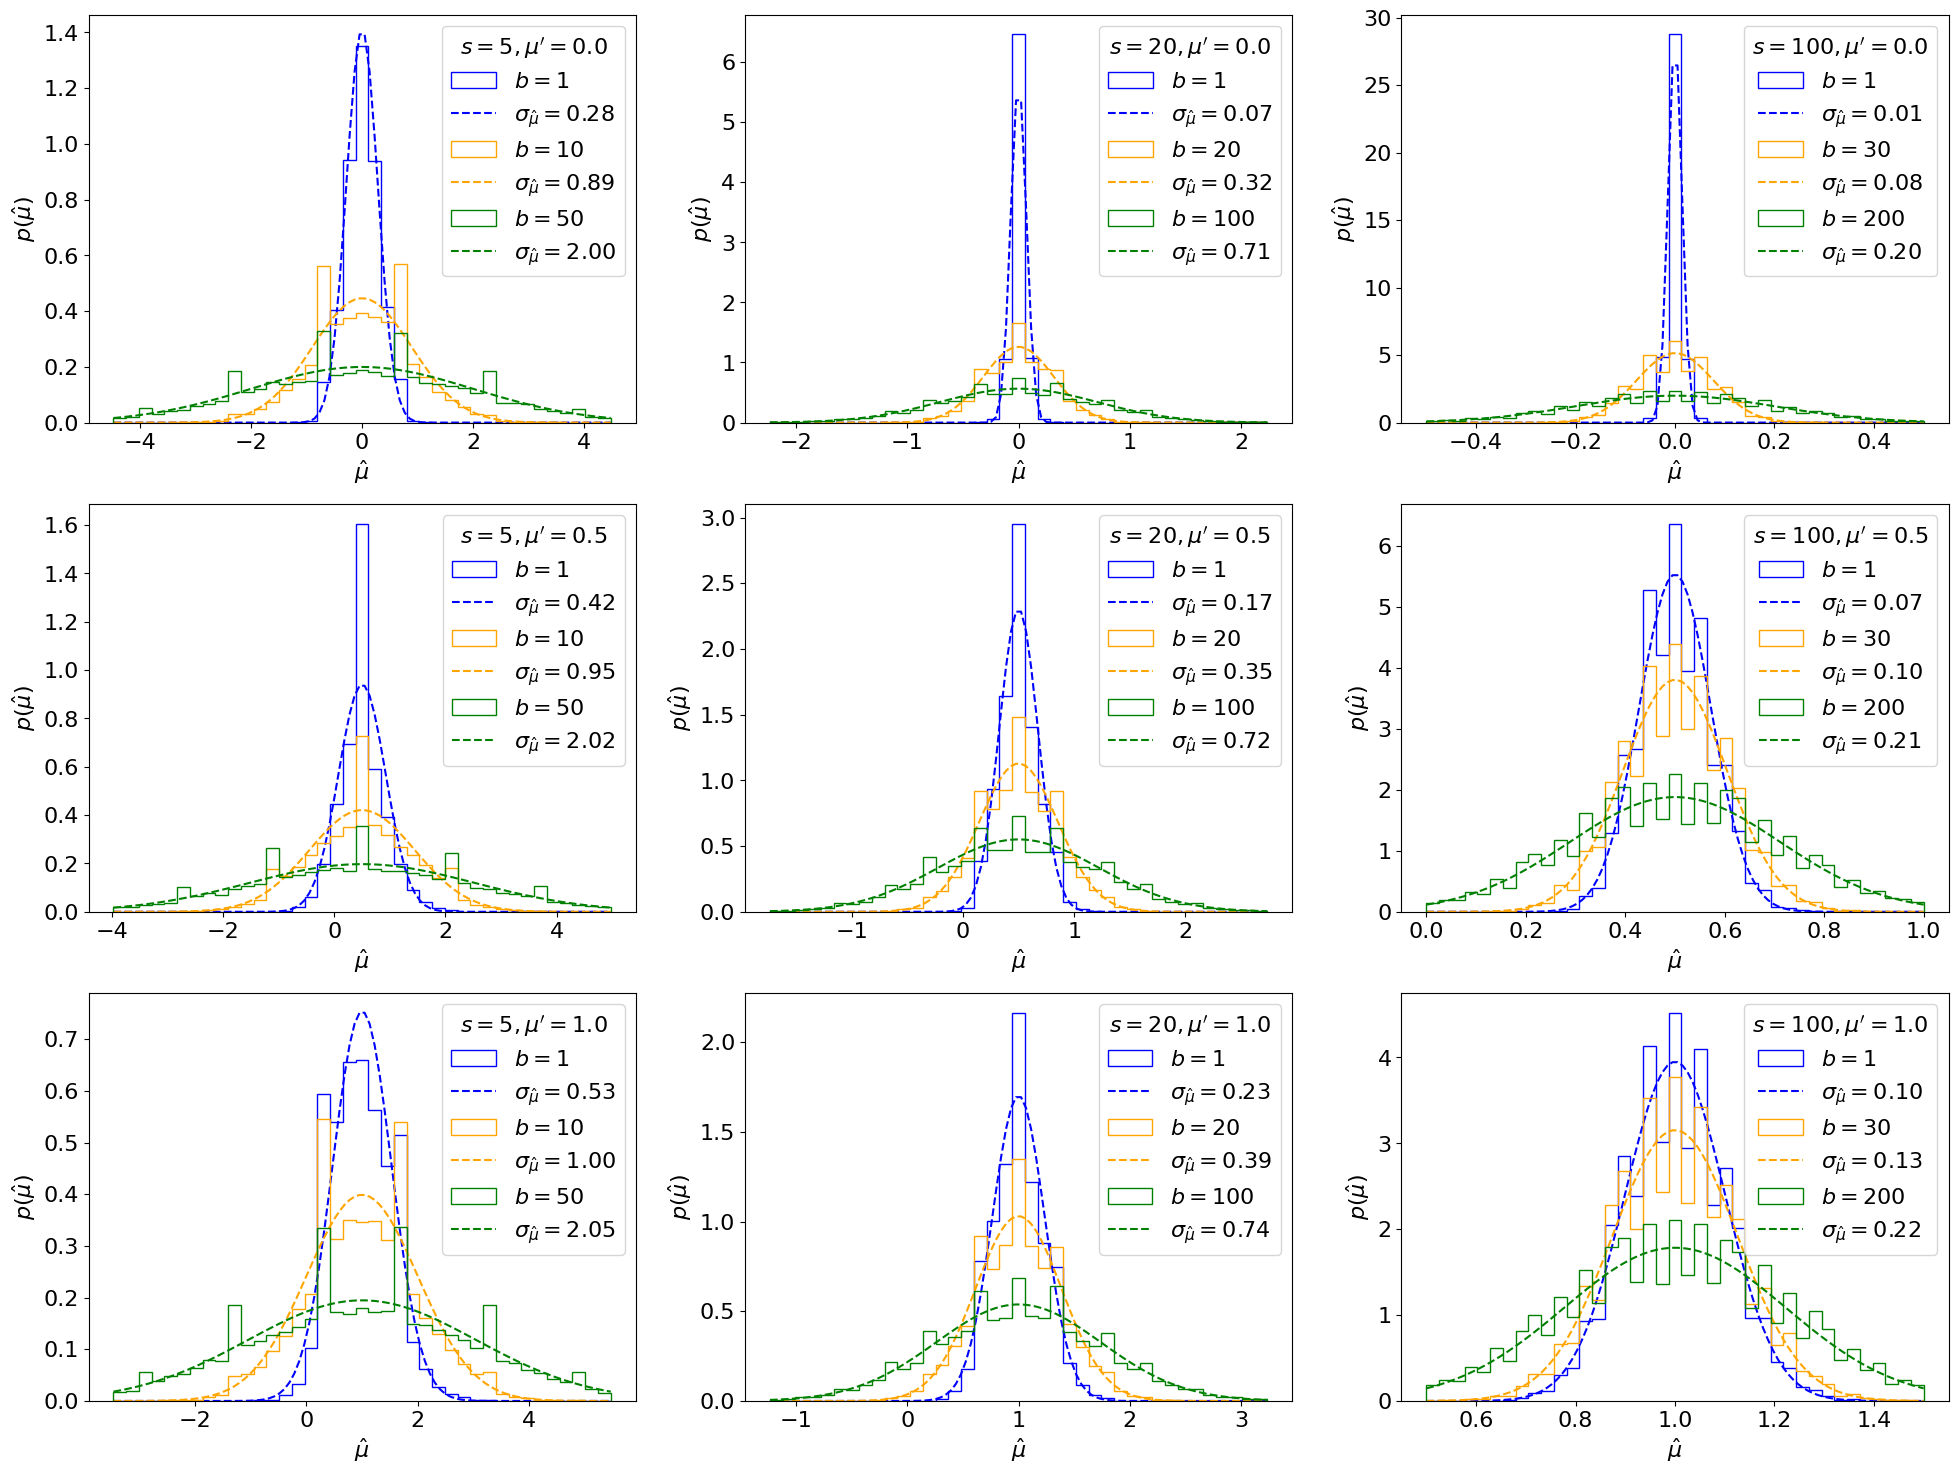
\includegraphics[width=\textwidth]{figures/05-asymptotic-mle/4.png}
\caption{Asymptotic (dotted lines) and toy-based (solid lines) distributions, using 30,000 toys each, of the MLE of $\mu$ for different $s$, $b$, and true signal strengths $\mu'$.}
\label{fig:p_mle_asym}
\end{figure}

We can also check the total per-bin errors between the asymptotic form and the toy-based distributions directly, as shown in Figure~\ref{fig:mle_errors} (for $\mu' = 1$ only).
Indeed, this confirms that the error scales as $\sim \frac{1}{\sqrt{s}}$ and $\sim \frac{1}{\sqrt{b}}$, as claimed above.

\begin{figure}[htb]
\centering
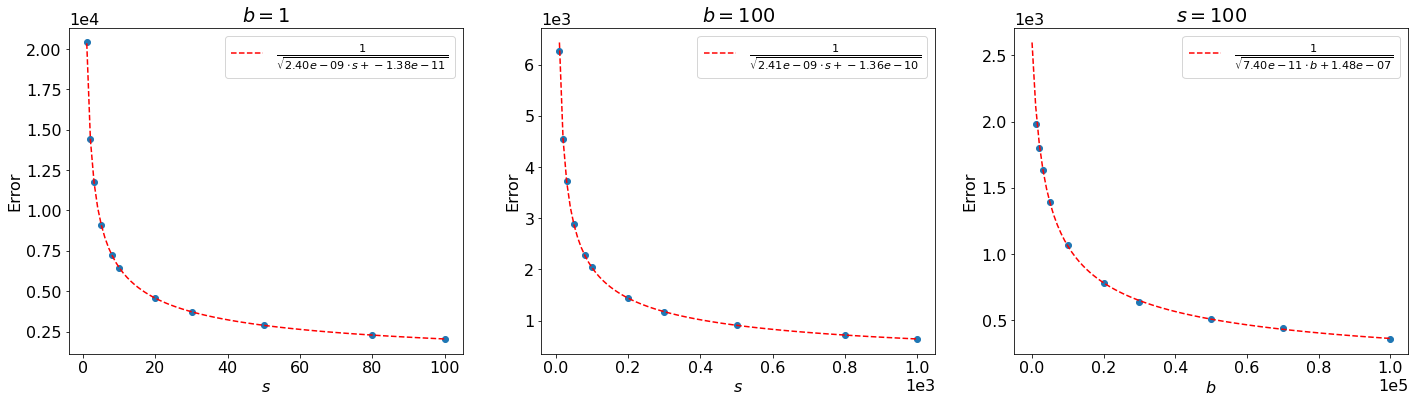
\includegraphics[width=\textwidth]{figures/05-asymptotic-mle/5.png}
\caption{Error between the sampled toy distributions, using 50,000 toys each, and the asymptotic distributions of the MLE of $\mu$ for different $s$ and $b$ (blue), with $1/\sqrt{N}$ fits in red.}
\label{fig:mle_errors}
\end{figure}


\section{Numerical estimation and the Asimov dataset}
\label{sec:pmle_asimov}

In this section, because of the simplicity of our data model, we were able to derive the Fisher information $\mathcal I$ and, hence, the asymptotic form of $\hat \mu$ analytically.
In general, this is not possible and we typically have to minimize $l$, find its second derivatives, and solve Eq.~\ref{eq:fisher} etc. \textit{numerically} instead.

However, when calculating the Fisher information, how do we deal with the expectation value over the observed data ($n, m$ in our case)? Naively, this would require averaging over a bunch of generated toy $n, m$ values again, which defeats the purpose of using the asymptotic form of $\hat \mu$!

Instead, we can switch the order of operations in Eq.~\ref{eq:fisher},\footnote{We are able to do this because, as we saw above, the score is linear in $n$ for Poisson likelihoods.} rewriting it as:
\begin{equation}
  \mathcal I_{ij}(\mu, b) = - \mathbb E[\partial^i\partial^j l(\mu, b; n, m)] = - \partial^i\partial^j \mathbb E[l(\mu, b; n, m)] = -\partial^i\partial^j l(\mu, b; \mathbb E[n], \mathbb E[m]).
\label{eq:fisher_asimov}
\end{equation}

Importantly, this says we can find $\mathcal I$ by simply evaluating the likelihood for a dataset of observations equal to their expectation values under $\mu'$ instead of averaging over the distribution of observations and \textit{then} getting its second derivatives.

\begin{definition}
Such a dataset is called the \textbf{Asimov} dataset, and $L(\mu; \mathbb E[n], \mathbb E[m]) \equiv L_A$ is referred to as the ``Asimov likelihood''.\footnote{The \textit{Asimov} dataset is named after Isaac Asimov, the popular science fiction author, whose book \textit{Franchise} is about a supercomputer choosing a single person as the sole voter in the U.S. elections, because they can represent the entire population.}
\end{definition}



\chapter{Asymptotic form of the profile likelihood ratio}
\label{sec:asymptotic_plr}

We can now proceed to derive the asymptotic form of the sampling distribution $p(t_\mu|\mu')$ of the profile likelihood ratio test statistic $t_\mu$, under a ``true'' signal strength of $\mu'$.
This asymptotic form is extremely useful for simplifying the computation of (expected) significances, limits, and intervals; indeed, standard procedure at the LHC is to use it in lieu of toy-based, empirical distributions for $p(t_\mu|\mu')$.


\section{Asymptotic form of the profile likelihood ratio}

We start with deriving the asymptotic form of the profile likelihood ratio test statistic $t_\mu$ (Eq.~\ref{eq:ts}) by following a similar procedure to Section~\ref{sec:pmle_derivation} --- and using the results therein --- of Taylor expanding around its minimum at $\hat\mu$:\footnote{Note: this is not a rigorous derivation; it's just a way to motivate the final result, which is taken from Ref.~\cite{Cowan:2010js}.
(If you know of a better way, let me know!)}
\begin{align}
    t_\mu &= -2\ln\lambda(\mu) \\
         &= -2l(\mu, \hat{\hat{b}}(\mu)) + 2l(\hat\mu, \hat{b}) \\
         &\simeq
        \underbrace{-2l(\hat\mu, \hat{\hat{b}}(\hat\mu)) + 2l(\hat\mu, \hat{b})}_{\textcolor{blue}{\hat{\hat{b}}(\hat\mu)=\hat b \text{ so this is 0}}} -
        \underbrace{2l'(\hat\mu, \hat{\hat{b}}(\hat\mu))(\mu-\hat\mu)}_{\textcolor{blue}{l'(\hat\mu, \hat b) = 0}} - 2l''(\hat\mu, \hat{\hat{b}}(\hat\mu))\cdot\frac{(\mu-\hat\mu)^2}{2} \\
        &= -l''(\hat\mu, \hat b) \cdot (\mu-\hat\mu)^2 \\
        &= \underbrace{-\mathbb E[l''(\hat\mu, \hat b)]}_{\textcolor{blue}{\text{By law of large numbers}}} \cdot (\mu-\hat\mu)^2 \label{eq:asym_plr_l5} \\
        &= \underbrace{-\mathbb E[l''(\mu', b')]}_{\textcolor{blue}{\text{Since bias of MLEs $\sim$ 0}}} \cdot (\mu-\hat\mu)^2 \label{eq:asym_plr_l6} \\
        &= \underbrace{\mathcal I_{\mu\mu}(\mu', b')}_{\textcolor{blue}{\text{From definition of Fisher information}}} \cdot (\mu-\hat\mu)^2 \\
 \Rightarrow  & \underbrace{\boxed{t_\mu \simeq \frac{(\mu-\hat\mu)^2}{\sigma_{\hat\mu}^2}}}_{\textcolor{blue}{\text{Using } \sigma_{\hat\mu} \simeq \sqrt{\mathcal I^{-1}_{\mu\mu}(\mu', b')}}} + \mathcal O((\mu-\hat\mu)^3) + \mathcal O(\frac{1}{\sqrt N}).
\label{eq:plr_taylor}
\end{align}

Here, just like in Eq.~\ref{eq:taylorl}, we use the law of large numbers in Line~\ref{eq:asym_plr_l5} and take $l''(\hat\mu, \hat b)$ to asymptotically equal its expectation value under the true parameter values $\mu', b'$: $l''(\hat\mu, \hat b) \xrightarrow{\sqrt{N} >> 1} \mathbb E[l''(\hat\mu, \hat b)]$.
We then in Line~\ref{eq:asym_plr_l6} also use the fact that MLEs are generally unbiased estimators of the true parameter values in the large sample limit to say $\mathbb E[l''(\hat\mu, \hat b)] \xrightarrow{\sqrt{N} >> 1} \mathbb E[l''(\mu', b')]$.
Finally, in the last step, we use the asymptotic form of the MLE (Eq.~\ref{eq:asym_std_fisher}).


\section{Asymptotic form of \texorpdfstring{$p(t_\mu|\mu')$}{p(t\_µ|µ')}}

Now that we have an expression for $t_\mu$, we can consider its sampling distribution.
With a simple change of variables, the form of $p(t_\mu|\mu')$ should hopefully be evident:
recognizing that $\mu$ and $\sigma_{\hat\mu}^2$ are simply constants, while $\hat\mu$ we know is distributed as a Gaussian centered around $\mu'$ with variance $\sigma_{\hat\mu}^2$, let's define $\gamma \equiv \frac{\mu-\hat\mu}{\sigma_{\hat\mu}}$, so that
\begin{align}
    t_\mu &\simeq \frac{(\mu-\hat\mu)^2}{\sigma_{\hat\mu}^2} = \gamma^2, \\
    \gamma &\sim \mathcal N \bigg(\frac{\mu - \mu'}{\sigma_{\hat\mu}}, 1 \bigg).
\label{eq:plr_gamma}
\end{align}

For the special case of $\mu = \mu'$, we can see that $t_\mu$ is simply the square of a standard normal random variable, which is the definition of the well-known $\chi^2_k$ distribution with $k=1$ degrees of freedom (DoF):
\begin{equation}
    p(t_\mu|\mu) \sim \chi^2_1.
\label{eq:chi2}
\end{equation}

In the general case where $\mu$ may not $ = \mu'$, $t_\mu$ is the square of random variable with unit variance but \textit{non-zero mean}.
This is distributed as the similar, but perhaps less well-known, \textbf{non-central chi-squared $\chipt_k(\Lambda)$}, again with 1 DoF, and with a ``non-centrality parameter''
\begin{align}
    \Lambda = \bar\gamma^2 &= \bigg(\frac{\mu - \mu'}{\sigma_{\hat\mu}}\bigg)^2,
  \label{eq:Lambda} \\
    p(t_\mu|\mu') &\sim \chipt_1(\Lambda).
  \label{eq:noncentralchi2}
\end{align}

The ``central'' vs. non-central chi-squared distributions are visualized in Figure~\ref{fig:noncentralchi2} for $k = 1$.
We can see that $\chipt_k(\Lambda)$ simply shifts towards the right as $\Lambda$ increases (at $\Lambda = 0$ it is a regular central $\chi^2$).
As $\Lambda \rightarrow \infty$, $\chipt_k(\Lambda)$ becomes more and more like a normal distribution with mean $\Lambda$.\footnote{More information can be found in e.g. Ref.~\cite{enwiki:1256854724}.
}

\begin{figure}[htb]
  \centering
  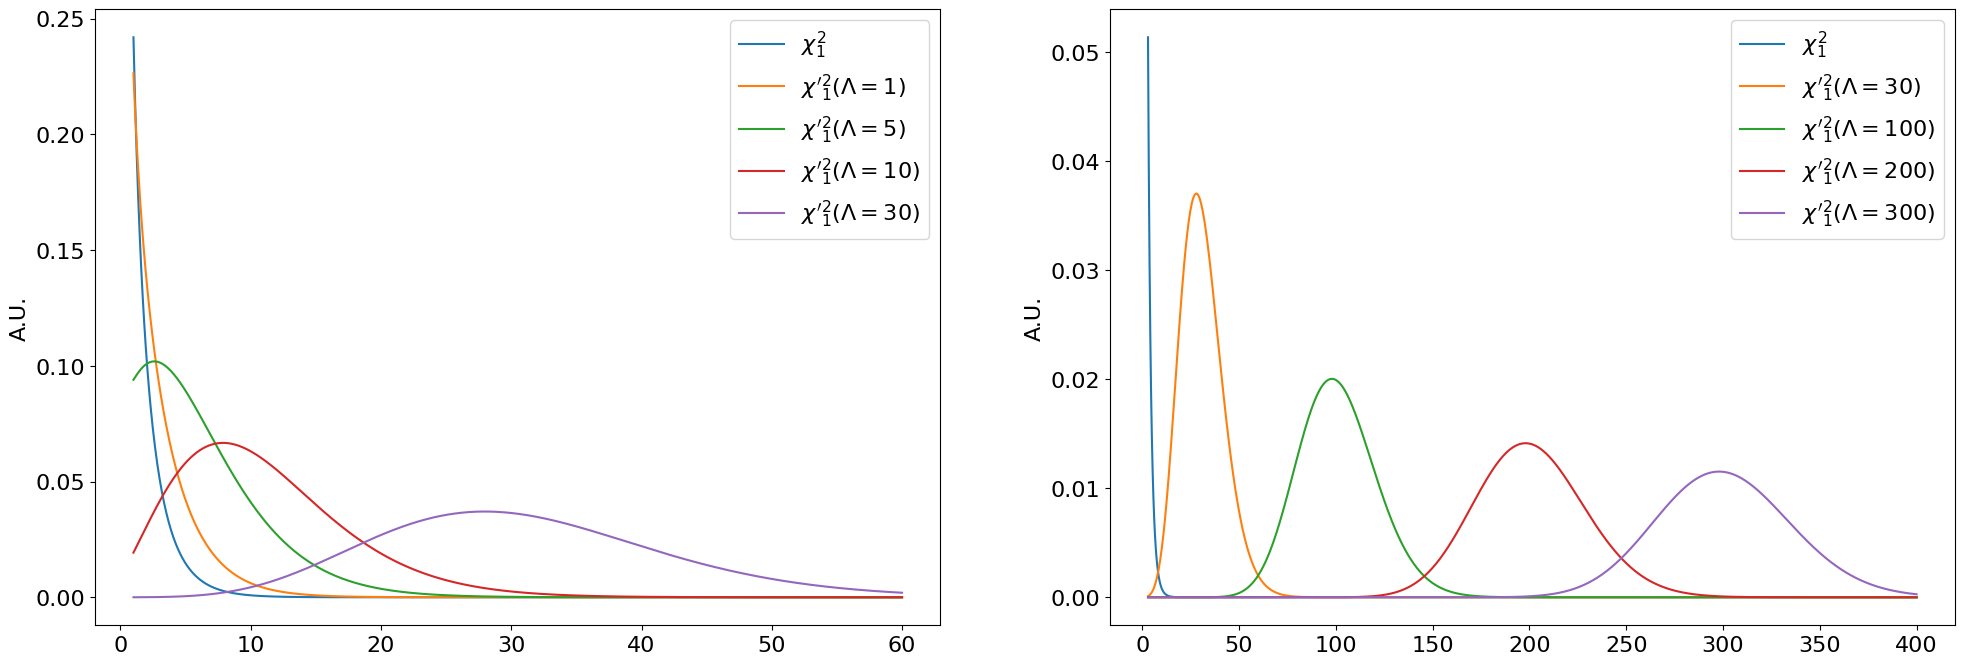
\includegraphics[width=\textwidth]{figures/06-asymptotic-plr/1.png}
  \caption{Central $\chi^2_k$ and non-central $\chipt_k(\Lambda)$ distributions for $\Lambda$ between $1-30$ (left) and $30-300$ (right).}
  \label{fig:noncentralchi2}
\end{figure}

By extending the derivation in Eq.~\ref{eq:plr_taylor} to multiple POIs, one can find the simple generalization to multiple POIs $\cvec\mu$:
\begin{equation}
p(t_\mu|\mu') \sim \chipt_k(\Lambda),
\label{eq:chi2multipois}
\end{equation}
where the DoF $k$ are equal the number of POIs $\dim\cvec\mu$, and
\begin{equation}
\Lambda = (\cvec\mu - \cvec\mu')^T \cdot \tilde{\mathcal I}^{-1}(\cvec\mu') \cdot (\cvec\mu - \cvec\mu'),
\label{eq:Lambdamultipois}
\end{equation}
where $\tilde{\mathcal I}^{-1}$ is $\mathcal I^{-1}$ restricted only to the components corresponding to the POIs.


\section{Estimating \texorpdfstring{$\sigma_{\hat\mu}^2$}{σ2}}

The critical remaining step to understanding the asymptotic distribution of $t_\mu$ is estimating $\sigma_{\hat\mu}^2$ to find the non-centrality parameter $\Lambda$ in Eq.~\ref{eq:Lambda}.
We now discuss two methods to do this.

\subsection{Method 1: Inverting the Fisher information / covariance matrix}

The first method is simply using $\sigma_{\hat\mu} \simeq \sqrt{\mathcal I^{-1}_{\mu\mu}(\mu', b')}$ as in Section~\ref{sec:asymptotic_mle}.\footnote{More generally, we'd need $\tilde{\mathcal I}^{-1}$ for Eq.~\ref{eq:Lambdamultipois}.}
This is shown in Figure~\ref{fig:ptmu_asym1} for our counting experiment, using the analytic form for $\sigma_{\hat\mu}$ from Eq.~\ref{eq:asymstd}.
We can see that this asymptotic approximation agrees well with the true distribution for some range of parameters, but can deviate significantly for others, as highlighted especially in the right plot.

\begin{figure}[htb]
  \centering
  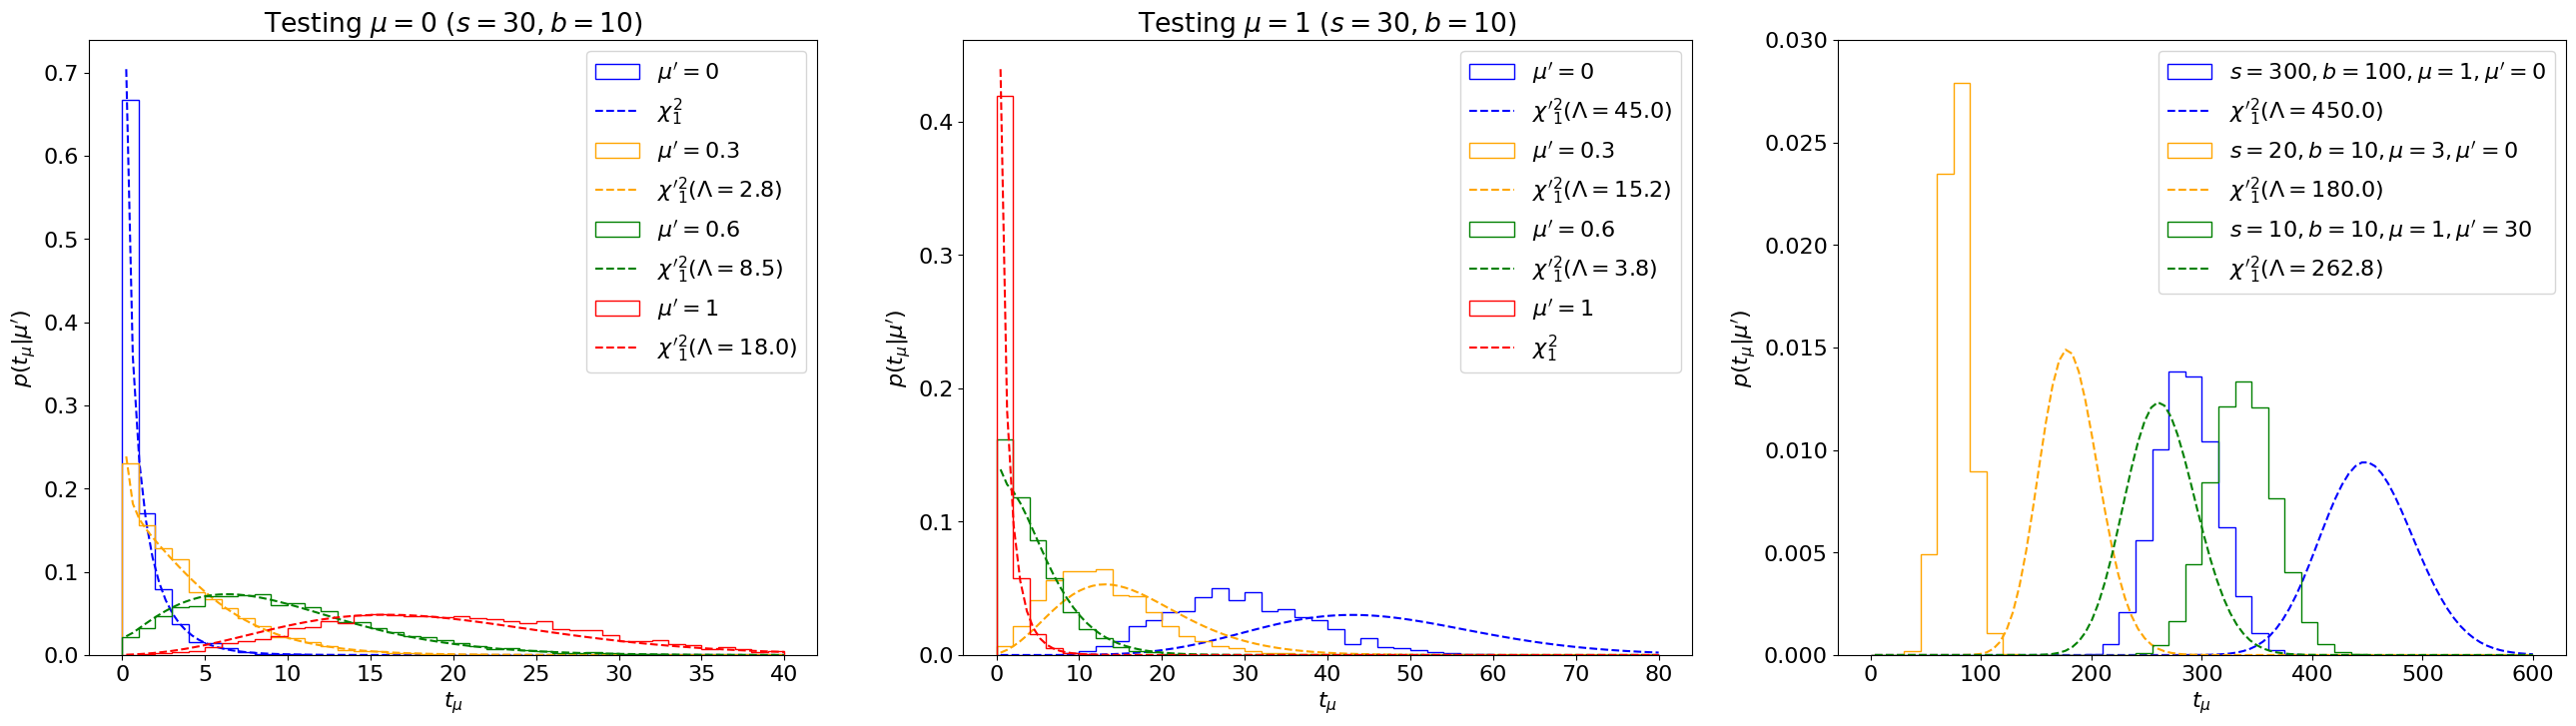
\includegraphics[width=\textwidth]{figures/06-asymptotic-plr/2.png}
  \caption{Comparing the distribution $p(t_\mu|\mu')$ (solid) with non-central $\chipt_1(\Lambda)$ distributions (dotted) for a range of $s, b, \mu, \mu'$ values, with $\sigma^2_{\hat\mu}$ estimated using the inverse of the Fisher information matrix.}
  \label{fig:ptmu_asym1}
\end{figure}


\subsection{Interlude on Asimov dataset}

While we are able to find the analytic form for $\sqrt{\mathcal I^{-1}_{\mu\mu}(\mu', b')}$ easily for our simple counting experiment, in general it has to be calculated numerically.
As introduced in Section~\ref{sec:pmle_asimov}, to handle the expectation value under $\mu', b'$ in Eq.~\ref{eq:fisher_matrix}, we can make use of the \textbf{Asimov dataset}, where the observations $n_A$, $m_A$ are taken to be their expectation values under $\mu', b'$, simplifying the calculation of $\mathcal I$ to Eq.~\ref{eq:fisher_asimov}.

Explicitly, for our counting experiment (Eq.~\ref{eq:pois3}), the Asimov observations are simply
\begin{align}
n_A &= \mathbb E[n] = \mu' s + b', \\
m_A &= \mathbb E[m] = b'.
\label{eq:asimov_data}
\end{align}
We'll now consider a second powerful use of the Asimov dataset to estimate $\sigma^2_{\hat\mu}$.

\subsection{Method 2: The ``Asimov sigma'' estimate}

Putting together Eqs.~\ref{eq:mles} and~\ref{eq:asimov_data}, we can derive a nice property of the Asimov dataset: the MLEs $\hat\mu$, $\hat b$ equal the true values $\mu'$, $b'$:
\begin{align}
    \hat b &= m_A = b' \\
    \hat \mu &= \frac{n_A - m_A}{s} = \frac{\mu's + b' - b'}{s} = \mu'.
\label{eq:asimov_mles}
\end{align}
Thus, $t_\mu$ evaluated for the Asimov dataset is exactly the non-centrality parameter $\Lambda$ that we are after!
\begin{equation}
    t_{\mu, A} \simeq \bigg (\frac{\mu-\hat\mu}{\sigma_{\hat\mu}}\bigg)^2 = \bigg (\frac{\mu-\mu'}{\sigma_{\hat\mu}}\bigg)^2 = \Lambda.
\label{eq:tmuasimov}
\end{equation}
While, not strictly necessary to obtain the asymptotic form for $p(t_\mu|\mu')$, we can also invert this to estimate $\sigma_{\hat\mu}$, as
\begin{equation}
    \sigma_A \simeq \frac{(\mu-\mu')^2}{t_{\mu, A}},
\label{eq:asimov_sigma}
\end{equation}
where $\sigma_A$ is known as the ``Asimov sigma''.

The asymptotic distributions using $\Lambda = t_{\mu, A}$ are plotted in Figure~\ref{fig:ptmu_asym2}.
We see that this estimate matches the sampling distributions very well, even for cases where the covariance-matrix-estimate failed!
Indeed, this is why estimating $\sigma_{\hat\mu} \simeq \sigma_A$ is the standard in LHC analyses, and that is the method we'll employ going forward.

Reference~\cite{Cowan:2010js} conjectures that this is because the Fisher-information-approach is restricted only to estimating the second-order term of Eq.~\ref{eq:plr_taylor}, while with $t_{\mu, A}$ we're matching the shape of the likelihood at the minimum which may be able capture some of the higher order terms as well.

\begin{figure}[htb]
  \centering
  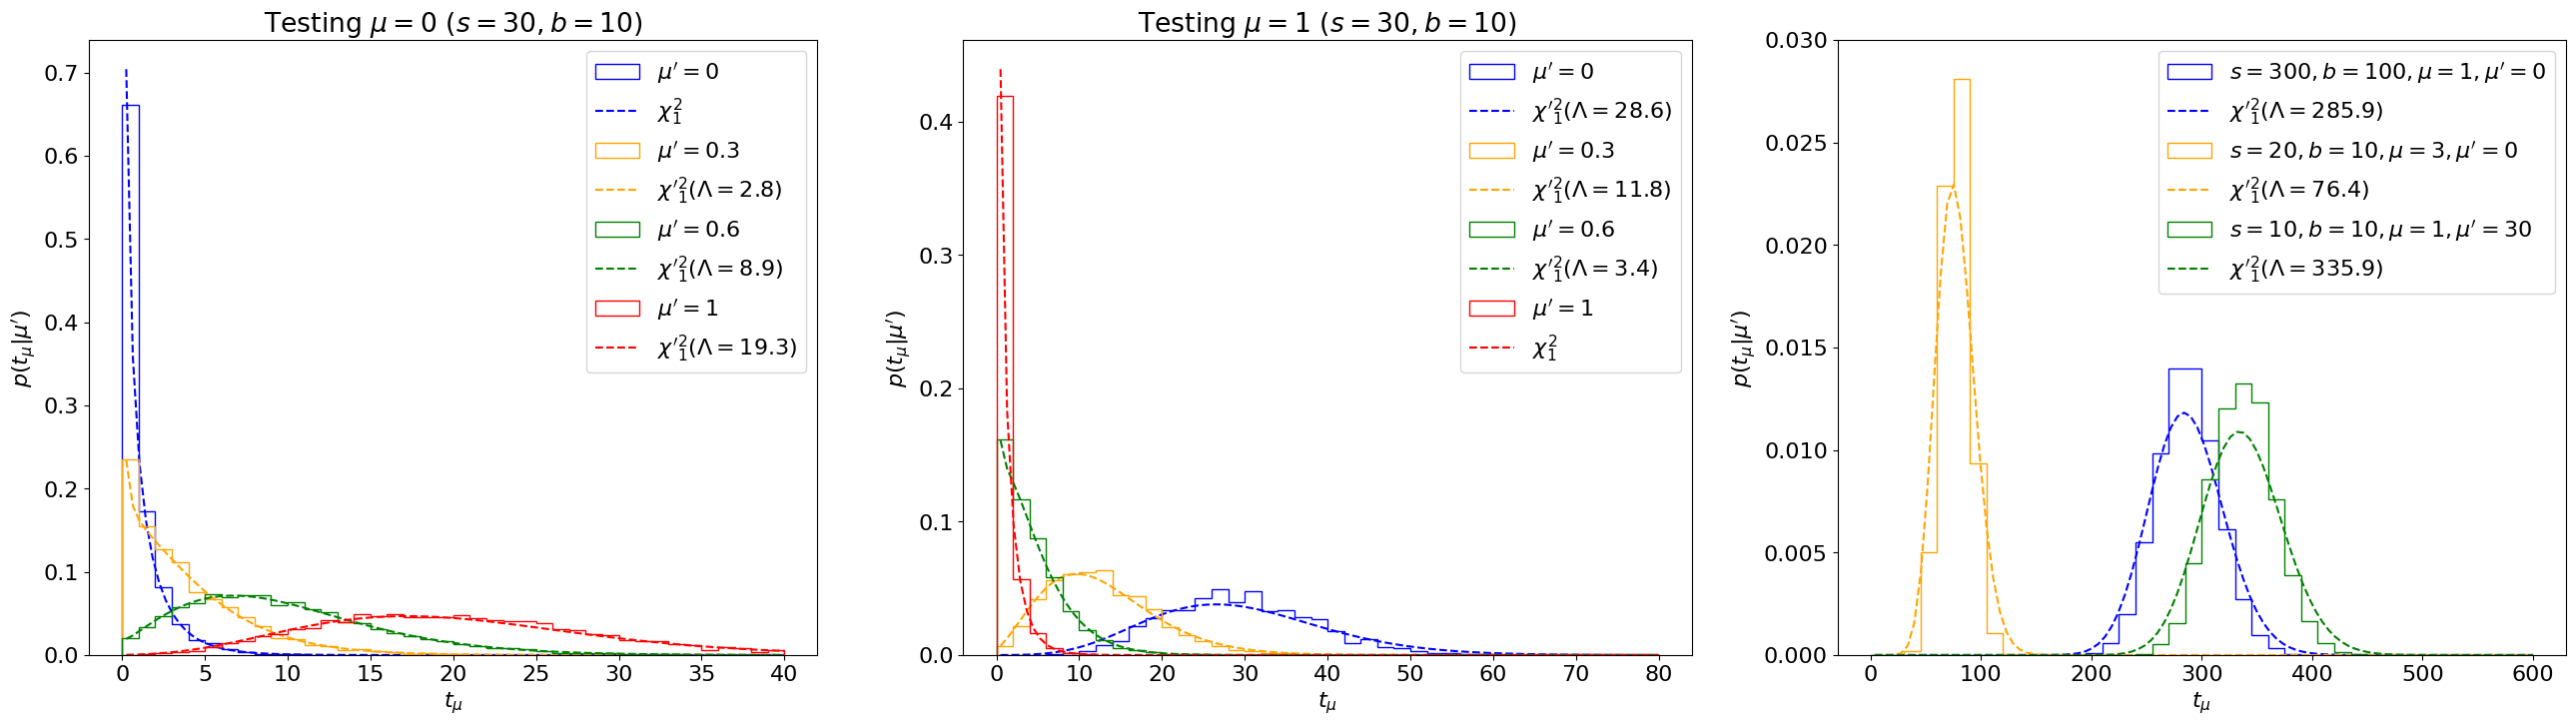
\includegraphics[width=\textwidth]{figures/06-asymptotic-plr/3.png}
  \caption{Comparing the sampling distribution $p(t_\mu|\mu')$ with non-central $\chipt_1(\Lambda)$ distributions for a range of $s, b, \mu, \mu'$ values, with the Asimov sigma estimation for $\sigma^2_{\hat\mu}$.}
  \label{fig:ptmu_asym2}
\end{figure}


Despite the pervasive use of the asymptotic formula at the LHC, it's important to remember that it's an \textit{approximation}, only valid for large statistics.
Figure~\ref{fig:ptmu_asym3} shows it breaking down for $s, b \lesssim 10$ below.

\begin{figure}[htb]
  \centering
  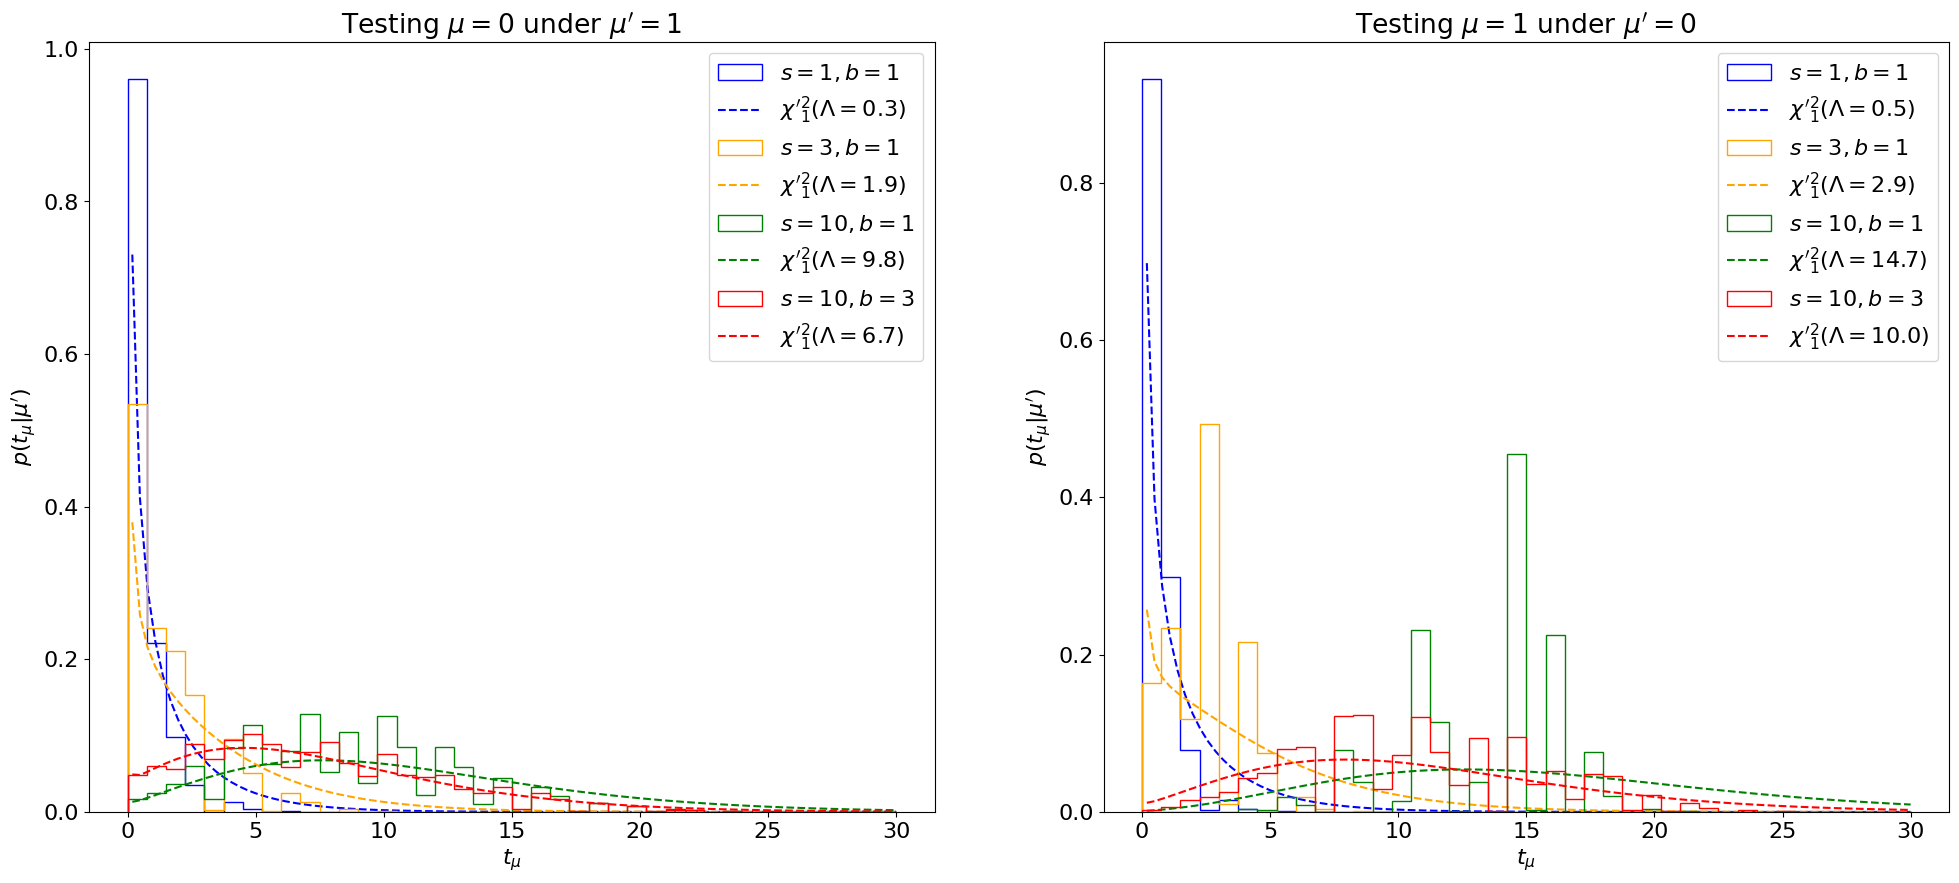
\includegraphics[width=\textwidth]{figures/06-asymptotic-plr/4.png}
  \caption{Comparing the sampling distribution $p(t_\mu|\mu')$ with non-central $\chipt_1(\Lambda)$ distributions for different $s, b \leq 10$, showing the break-down of the $\sigma_A$ approximation for $\sigma^2_{\hat\mu}$ at low statistics.}
  \label{fig:ptmu_asym3}
\end{figure}

\section{The PDF and CDF}

The probability distribution function (PDF) for a $\chipt_k(\Lambda)$ distribution can be found in e.g. Ref.~\cite{enwiki:1256854724} for $k=1$:
\begin{equation}
    p(t_\mu|\mu') \simeq \chipt_1(\Lambda) = \frac{1}{2\sqrt{t_\mu}}\big(\varphi(\sqrt{t_\mu} - \sqrt\Lambda) + \varphi(\sqrt{t_\mu} + \sqrt\Lambda)\big),
\label{eq:ptmu_pdf}
\end{equation}
where $\varphi$ is the PDF of a standard normal distribution.
For $\mu = \mu' \Rightarrow \Lambda = 0$, this simplifies to:
\begin{equation}
    p(t_\mu|\mu) \simeq \chi^2 = \frac{1}{\sqrt{t_\mu}}\varphi(\sqrt{t_\mu}).
\label{eq:ptmu_pdf_special}
\end{equation}

The cumulative distribution function (CDF) for $k=1$ is:
\begin{equation}
    F(t_\mu|\mu') \simeq \Phi(\sqrt{t_\mu} - \sqrt\Lambda) + \Phi(\sqrt{t_\mu} + \sqrt\Lambda) - 1,
\label{eq:ptmu_cdf}
\end{equation}
where $\Phi$ is the CDF of the standard normal distribution.
For $\mu = \mu' \Rightarrow \Lambda = 0$, again this simplifies to:
\begin{equation}
    F(t_\mu|\mu) \simeq 2\Phi(\sqrt{t_\mu}) - 1.
\label{eq:ptmu_cdf_special}
\end{equation}
From Eq.~\ref{eq:pvalue}, we know the $p$-value $p_\mu$ of the observed $t_\mu^{\mathrm{obs}}$ under a signal hypothesis of $H_\mu$ is
\begin{equation}
    p_\mu = 1 - F(t_\mu^{\mathrm{obs}}|\mu) = 2(1 - \Phi(\sqrt{t_\mu^{\mathrm{obs}}})),
\label{eq:pmu_asym}
\end{equation}
with an associated significance
\begin{equation}
    Z = \Phi^{-1}(1-p_\mu) = \Phi^{-1}(2\Phi(\sqrt{t_\mu^{\mathrm{obs}}} - 1)
\label{eq:Z_asym}
\end{equation}


\section{Application to hypothesis testing}

Let's see how well this approximation agrees with the toy-based $p$-value we found in Example~\ref{ex:pvalue}.
For the same counting experiment example, where we expect $s = 10$ and observe $n_{\mathrm{obs}} = 20$, $m_{\mathrm{obs}} = 5$, we found the $p$-value for testing the $\mu = 1$ hypothesis $p_{\mu = 1} = 0.3$ (and the associated significance $Z = 0.52$).
Calculating $t_\mu^{\mathrm{obs}}$ for this example and plugging it into the asymptotic approximation from Eq.~\ref{eq:pmu_asym} gives:\footnote{Note that we're using $t_\mu$ here, not the alternative test statistic $\tilde{t_\mu}$; however, in this case since $\hat\mu > 0$, they are equivalent.}
\begin{align}
\label{eq:pmu_asym_example}
  &t_\mu^{\mathrm{obs}} = 1.08  \\
  &\Rightarrow p_{\mu = 1} = 2(1 - \Phi(\sqrt{1.08})) = 0.3 \\
  &\Rightarrow Z = 0.52.
\end{align}
We see that it agrees exactly!

The agreement more generally, with varying $s, \mu, n_{\mathrm{obs}}, m_{\mathrm{obs}}$, is plotted in Figure~\ref{fig:asym_significances}.
We observe generally strong agreement, except for low $n, m$ where, as expected, the asymptotic approximation breaks down.

\begin{figure}[htb]
  \centering
  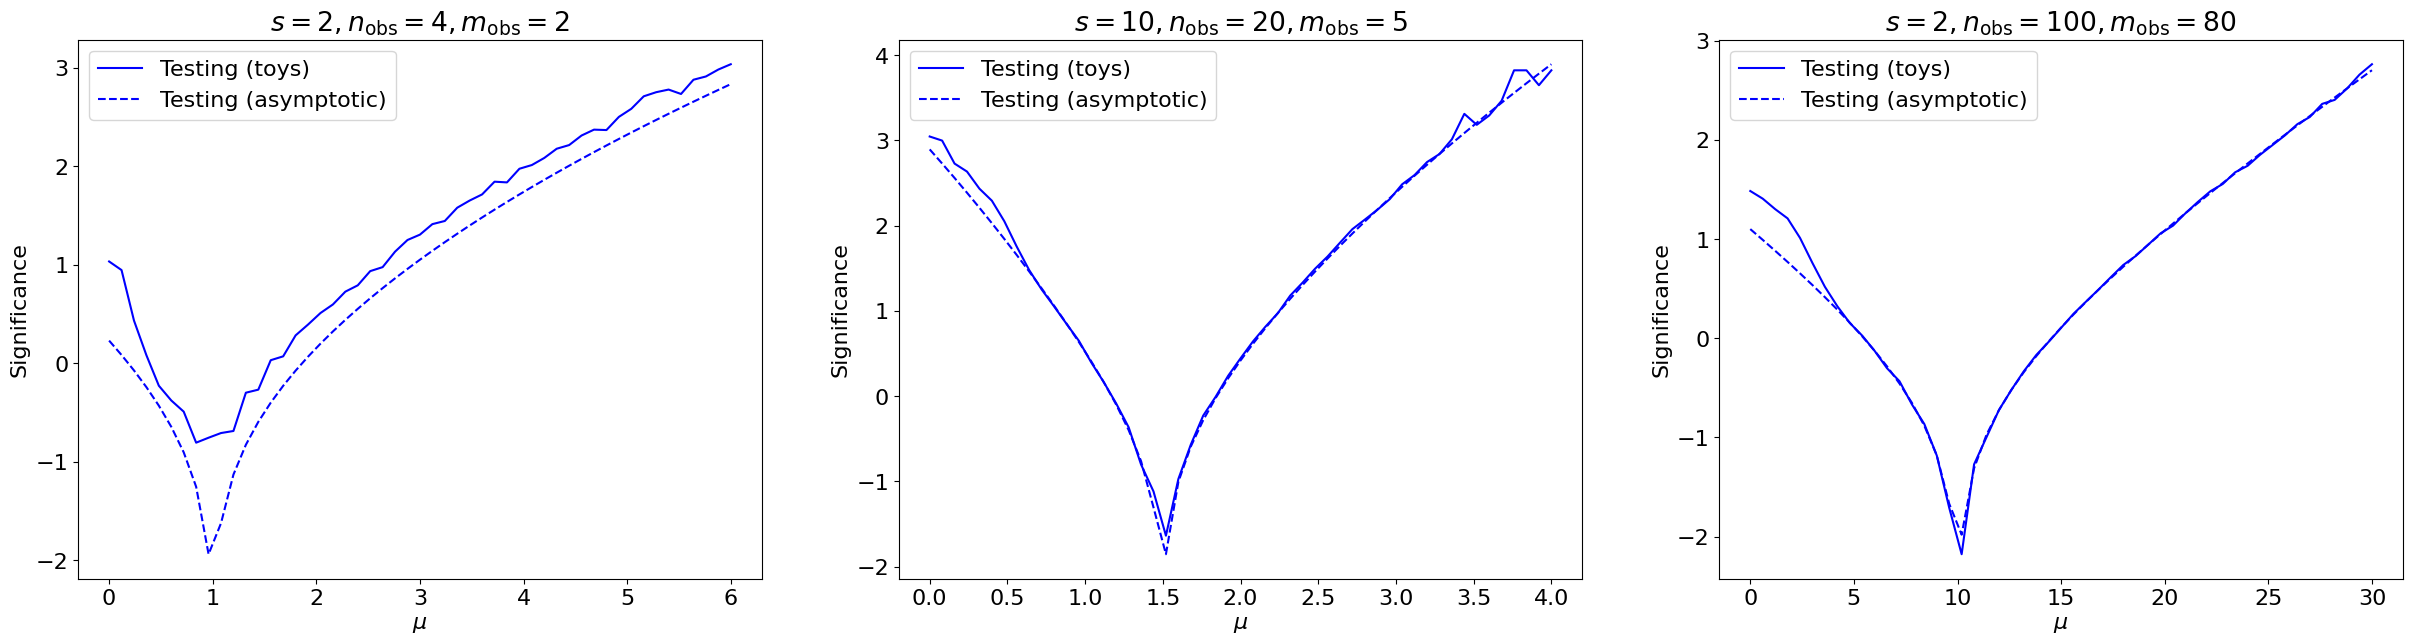
\includegraphics[width=\textwidth]{figures/06-asymptotic-plr/5.png}
  \caption[Comparing the significances, as a function of the signal strength $\mu$ of the hypothesis being tested, for simple counting experiments (Eq.~\ref{eq:pois3}) with different $s, n_{\mathrm{obs}}, m_{\mathrm{obs}}$'s.]{Comparing the significances, as a function of the signal strength $\mu$ of the hypothesis being tested, for simple counting experiments (Eq.~\ref{eq:pois3}) with different $s, n_{\mathrm{obs}}, m_{\mathrm{obs}}$'s, derived using $30,000$ toys each (solid) to estimate the $p(t_\mu|\mu)$ distribution vs. the asymptotic approximation (dashed).}
  \label{fig:asym_significances}
\end{figure}


\section{Summary}

We have been able to find the asymptotic form for the profile-likelihood-ratio test statistic $t_\mu \simeq \frac{(\mu-\hat\mu)^2}{\sigma_{\hat\mu}^2}$, which is distributed as a \textit{non-central chi-squared} ($\chipt_k(\Lambda)$) distribution.
We discussed two methods for finding the non-centrality parameter $\Lambda$, out of which the Asimov sigma $\sigma_A$ estimation generally performed better.
Finally, the asymptotic formulae were applied to simple examples of hypothesis testing to check the agreement with toy-based significances.
These asymptotic formulae can be extended to the alternative test statistics for positive signals $\tilde{t}_\mu$ and upper-limit-setting $\tilde{q}_\mu$, as in Ref.~\cite{Cowan:2010js}, to simplify the calculation of both observed and expected significances, limits, and intervals.
\end{doublespace}

\nocite{apsrev42Control}
\bibliography{bibliography}

\end{document}
